\chapter{具体需求}
\section{功能需求}

本子章节应描述软件产品的输入怎样被转换成输出。它描述了软件必须执行的基本动作。 

\subsection{URS\_Browse\_F01 浏览目录}

\subsubsection{介绍}

用户可以浏览不同音乐的类型、类别,同时可以查看专辑的详细信息,如描述、价格和歌曲列表等。根据用户所选的类型/类别,使用相应的查询方式访问关系数据库。

错误输入:当显示第一页时点击前一页,当显示最后一页时点击后一页;

非法条件:没有登录,直接浏览该页面。

无效输入:无

\begin{center} 
\begin{sideways}
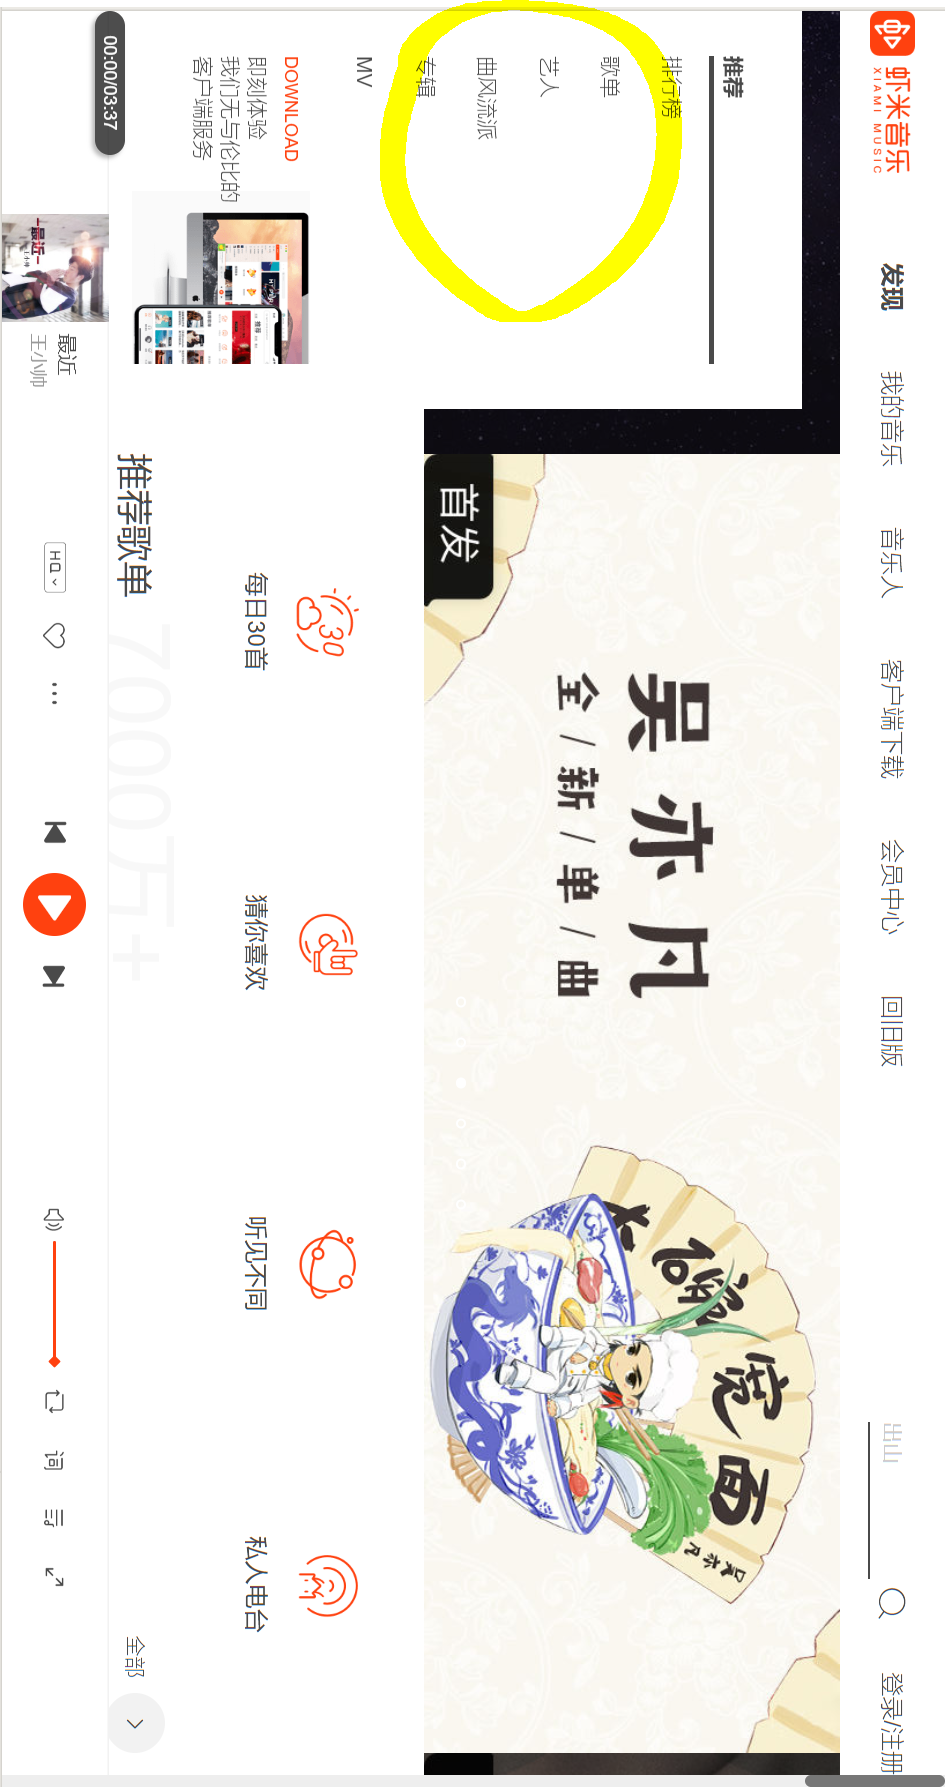
\includegraphics[width=0.5\textwidth]{./figures/capture.png} 
\end{sideways}
\end{center}
\subsubsection{输入}

输入:用户通过鼠标点选其中一个类型及其类别。


\subsubsection{处理}



A. 输入数据的有效性检测:不需要进行有效性检测,因为输入是通过鼠标在对应区域点击引起中断造成的。

B. 操作的确切次序:
\begin{adjustwidth}{2cm}{1cm}\qquad
	\begin{itemize}
		\item 中断事件发生
		\item 调用监听函数
		\item 函数对数据库发起查询请求
		\item 数据库接收到请求,并回送相关数据
		\item 监听函数接收到数据
		\item 刷新网页,将数据以合适的方式显示给用户
	\end{itemize}		
\end{adjustwidth}
 

C. 对异常情况的回应,例如:
\begin{adjustwidth}{2cm}{1cm}\qquad
	\begin{itemize}
		\item 溢出
		\item 通信失败
		\item 错误处理
	\end{itemize}		
\end{adjustwidth}

	发生以上错误时,函数体向网页返回错误代码,网页打印相应错误信息

D. 通过过程性sql指令向数据库传送查询请求
		
E. 对输出数据的有效性检测:

在监听函数接收到数据库传送过来的数据后,首先进行合法性检测,如果合法则令网页正常显示;如果数据不合法或不安全——返回错误代码,让网页打印错误信息;

\subsubsection{输出}

A. 输出描述:
\begin{itemize}
 \item	输出:动态网页显示
 \item	数量:1
 \item	度量单位:页
 \item	时序:无
 \item	包含精确度和容忍度的有效输出范围:无
 \item	对非法值的处理:打印错误信息
 \item	错误消息:当输出不合法时,打印网页不存在或者输入信息错误;
\end{itemize}
详细描述:
系统将显示所选类型及类别的商品列表和信息。商品列表将显示在product.aspx页面上,每个页面上将显示6张专辑,其余部分(如果有)将显示在下一页上。
这将使用“分页”功能执行,即每个product.aspx页面底部都会有一个名为“Previous”和“Next”的链接,以使客户能够转到下一页和上一页以查看产品。
客户的当前所在页面也将显示在每个页面上。
\subsection{URS\_Search\_F02 搜索音乐}

\subsubsection{介绍}
% \iffalse

% 逐条列出与本特性相关的功能需求。包括项目如何响应预期的错误输入,非法条件和无效输入。需求应该简明,完整,不含糊,可验证,必要的。 当需要的信息不确定的时候使用“待定”。
% \fi
本部分应用的目的是使客户能够在不浏览整个目录的情况下找到他选择的可用产品(音乐或者专辑)。
\begin{center} 
	\begin{sideways}
	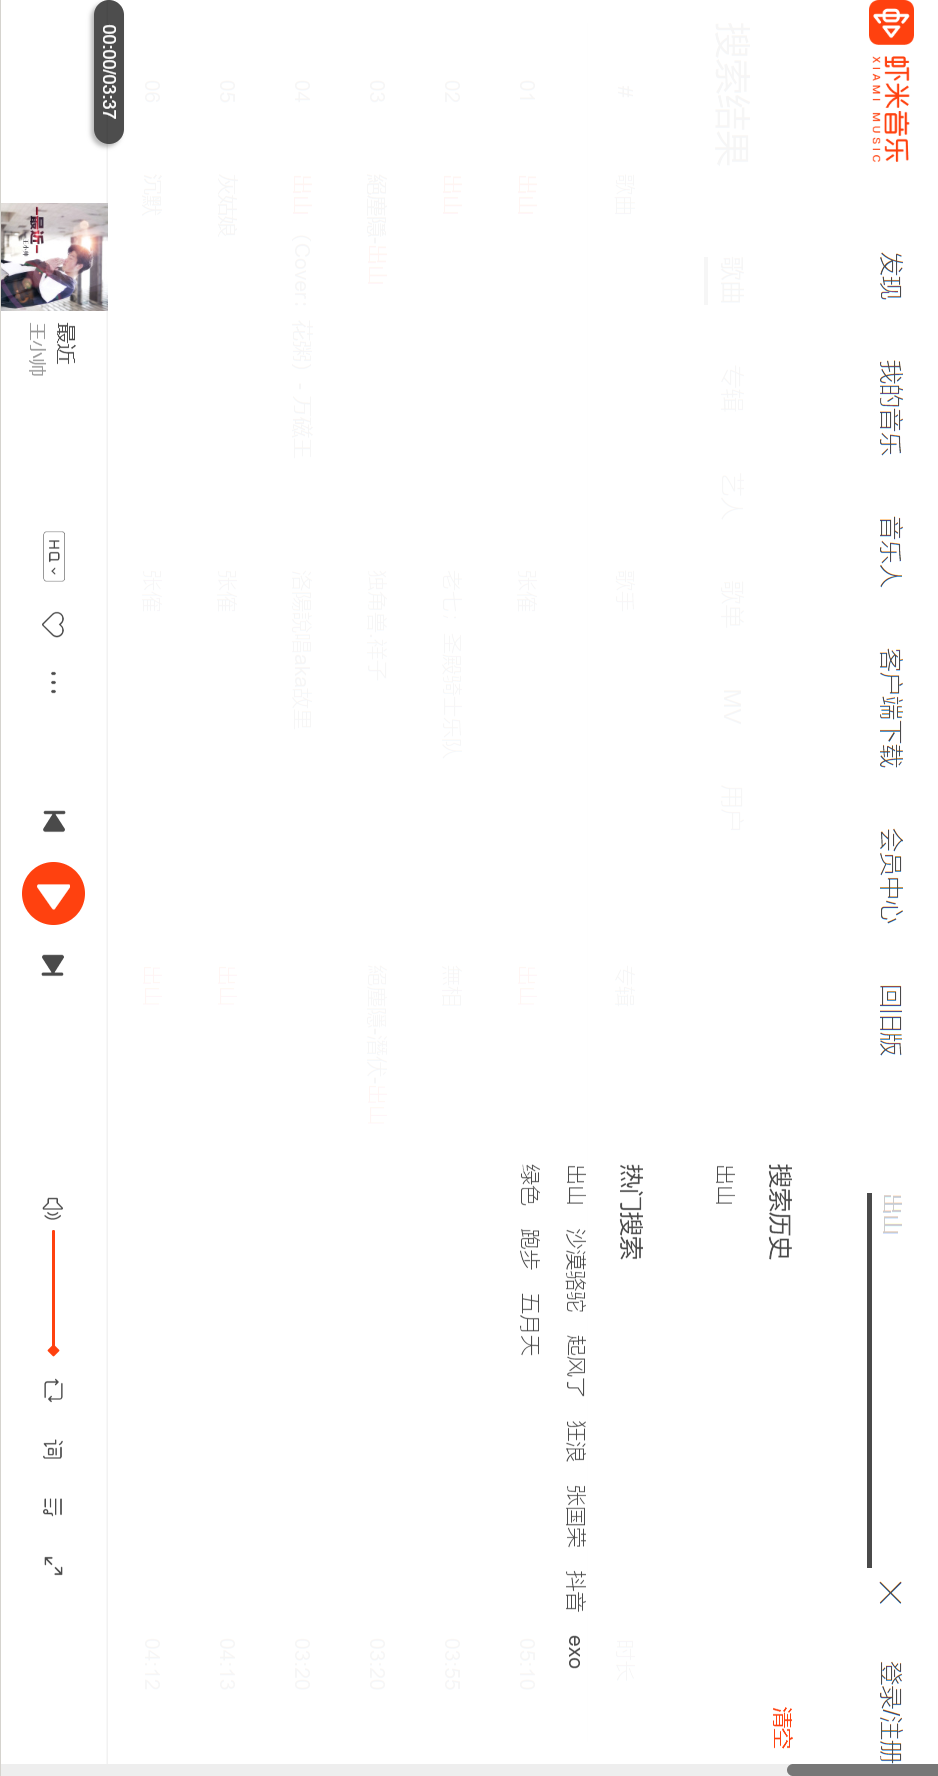
\includegraphics[width=0.5\textwidth]{./figures/capture2.png} 
	\end{sideways}
	\end{center}
	\begin{center} 
		\begin{sideways}
		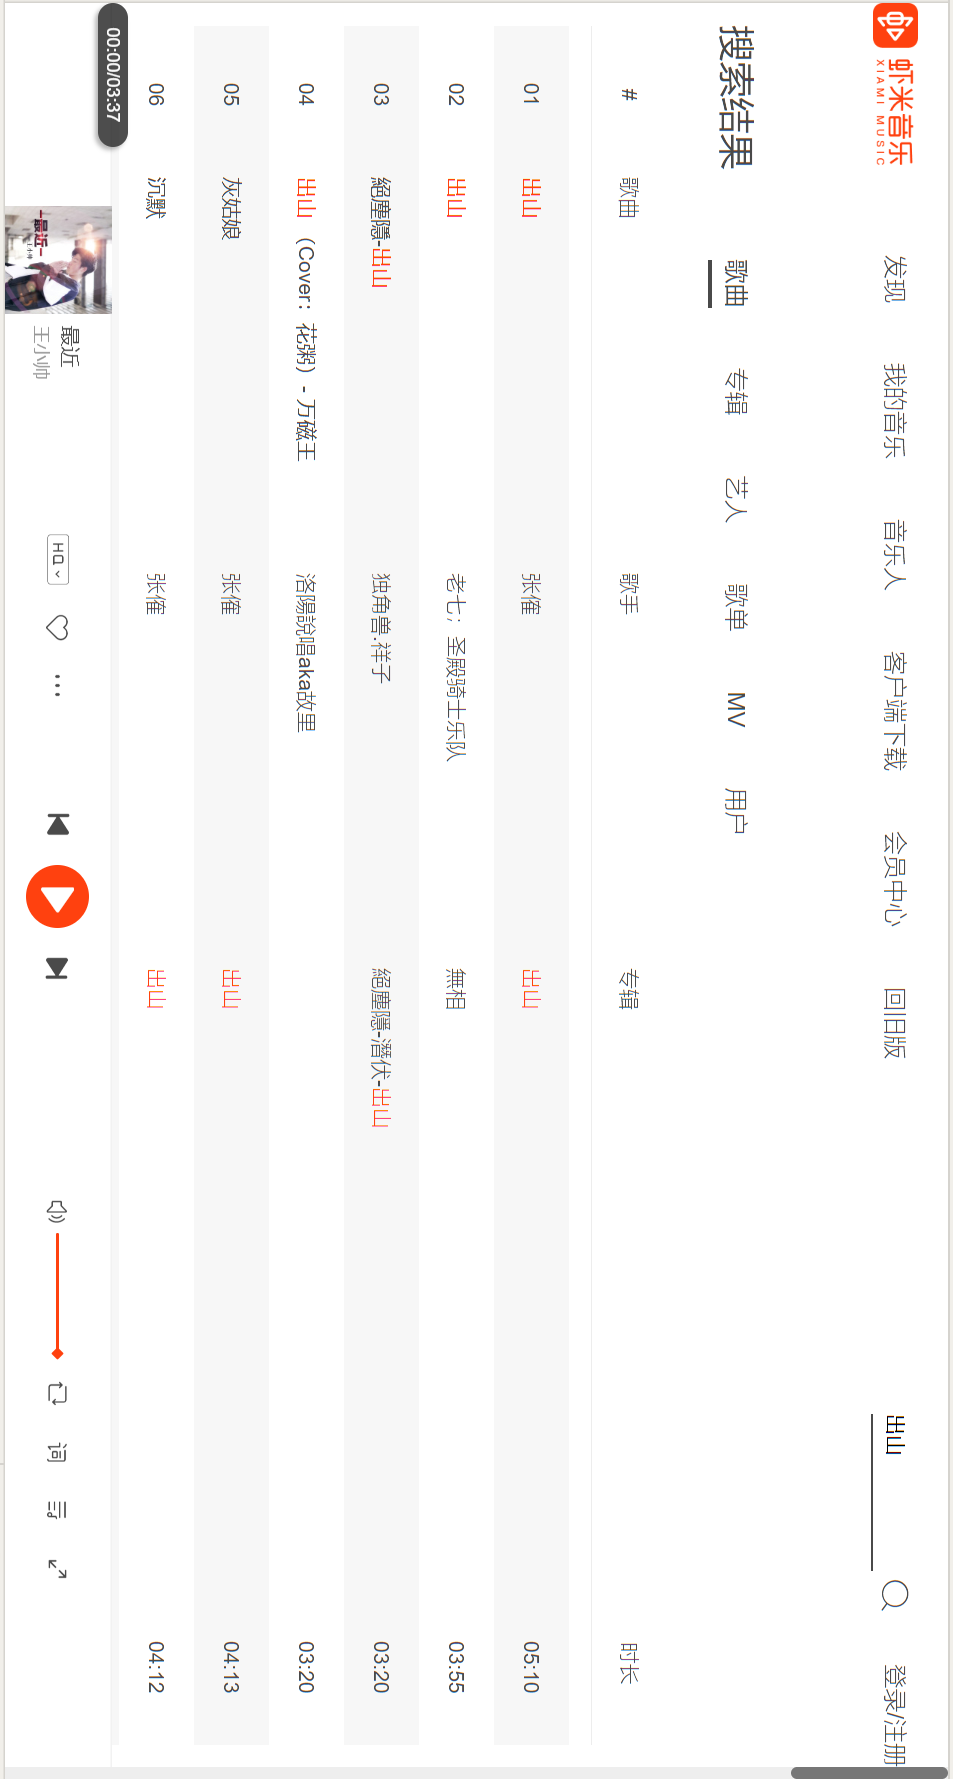
\includegraphics[width=0.5\textwidth]{./figures/capture3.png} 
		\end{sideways}
		\end{center}
输入:用户将点击每页顶部的“搜索”按钮。
用户可以在搜索文本框中输入任何文本,并可以选择让系统搜索他输入的所有单词并点击“搜索”按钮。
然后他可以选择输入音乐专辑/ CD的名称,艺术家,风格,格式和他/她选择的价格范围。
这会将用户重定向到显示所有匹配项目的页面; 否则将显示相应的消息。

\subsubsection{处理}



A. 输入数据的有效性检测:不需要进行有效性检测,因为输入是通过鼠标在对应区域点击引起中断造成的。

B. 操作的确切次序:
\begin{adjustwidth}{2cm}{1cm}\qquad
	\begin{itemize}
		\item 中断事件发生
		\item 调用监听函数
		\item 用户重定向到Search.aspx网页
		\item 用户在搜索框中输入文本
		\item 文本输入完毕后,按下回车键或者点击搜索按钮
		\item 将输入文本转化为数据库查询,传送到服务器端
		\item 服务器回送数据到客户端
		\item 监听器感知到回送数据,刷新网页
	\end{itemize}		
\end{adjustwidth}
 

C. 对异常情况的回应,例如:
\begin{adjustwidth}{2cm}{1cm}\qquad
	\begin{itemize}
		\item 溢出
		\item 通信失败
		\item 错误处理
	\end{itemize}		
\end{adjustwidth}

	发生以上错误时,函数体向网页返回错误代码,网页打印相应错误信息

D. 通过过程性sql指令向数据库传送查询请求
		
E. 对输出数据的有效性检测:

在监听函数接收到数据库传送过来的数据后,首先进行合法性检测,如果合法则令网页正常显示;如果数据不合法或不安全——返回错误代码,让网页打印错误信息;

\subsubsection{输出}
\begin{itemize}
	\item	输出:动态网页显示
	\item	数量:1
	\item	度量单位:页
	\item	时序:无
	\item	包含精确度和容忍度的有效输出范围:无
	\item	对非法值的处理:打印错误信息
	\item	错误消息:当输出不合法时,打印网页不存在或者输入信息错误;
   \end{itemize}
   详细描述:
   如果用户输入无效(即用户未输入任何所需选项),将显示相应的错误消息。如果输入有效,将显示一条消息,要求用户确认需要搜索的相应产品信息。如果没有匹配项,系统也将显示相应的消息。
  
 
   \subsection{URS\_Share\_F03 分享(专辑/歌单/单曲)}

   \subsubsection{介绍}
   
   用户在专辑页面、歌单页面中,或者在播放栏中点击分享按键
   
   错误输入:因为是鼠标点击输入,所以不存在错误输入
   
   非法条件:没有登录,直接点击分享
   
   无效输入:无
   \begin{center} 
	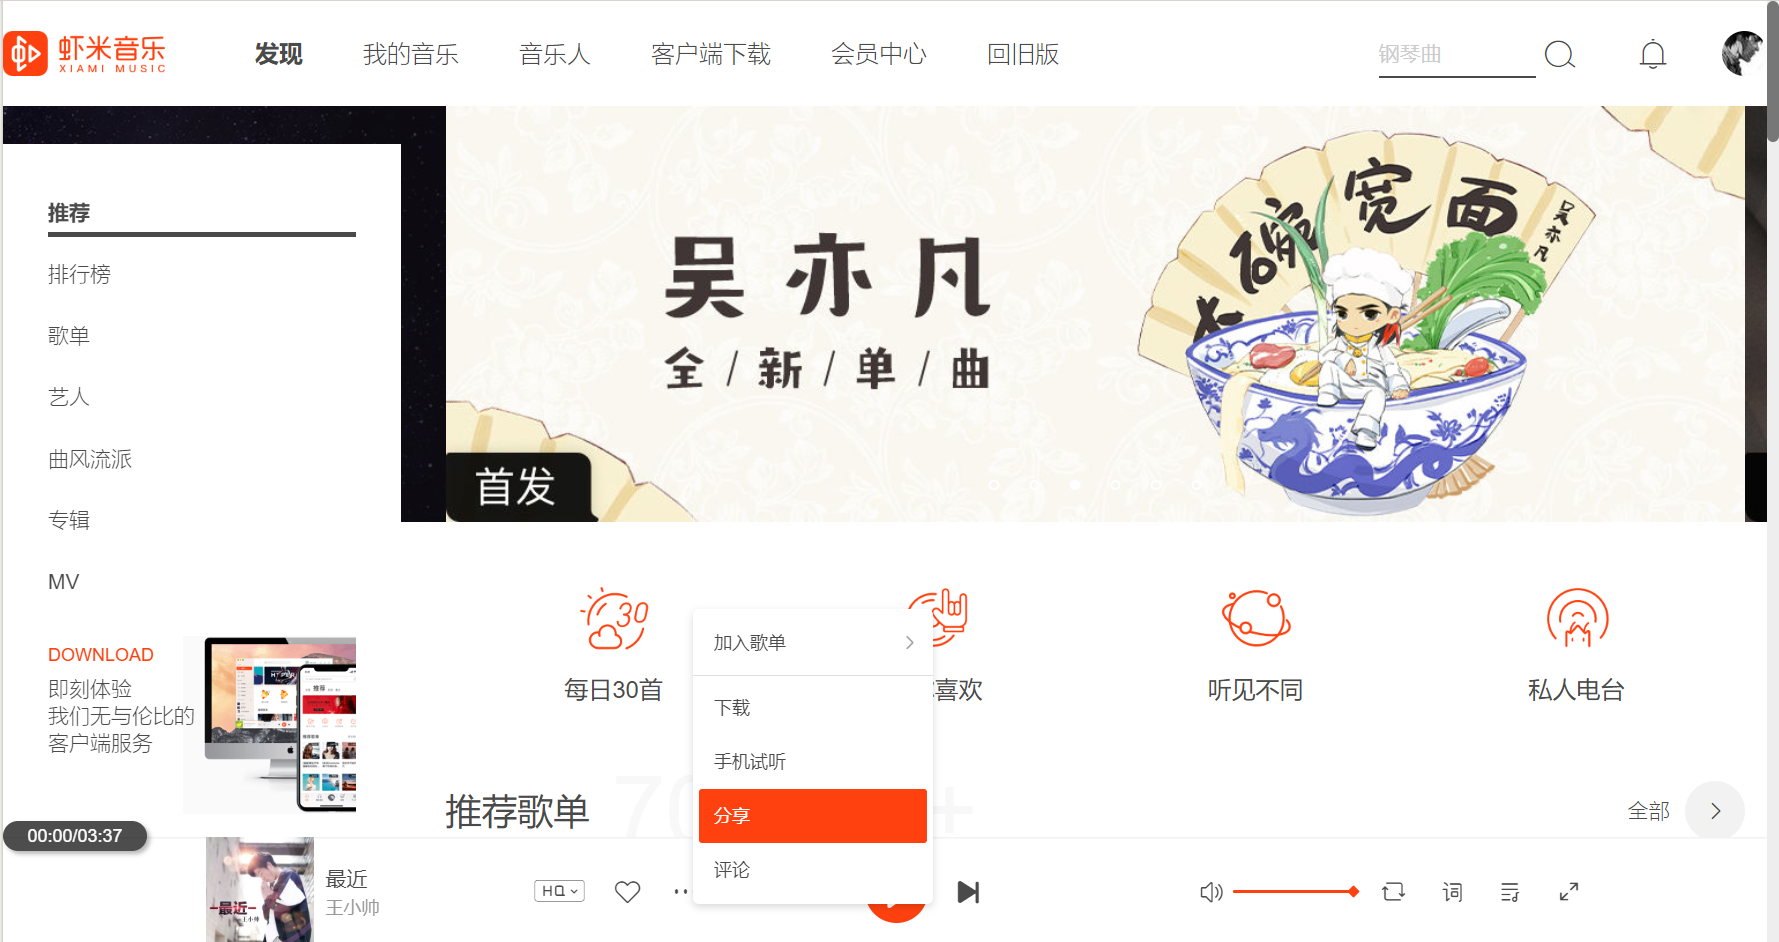
\includegraphics[width=0.5\textwidth]{./figures/capture5.png} 

	\end{center}
	\begin{center} 
		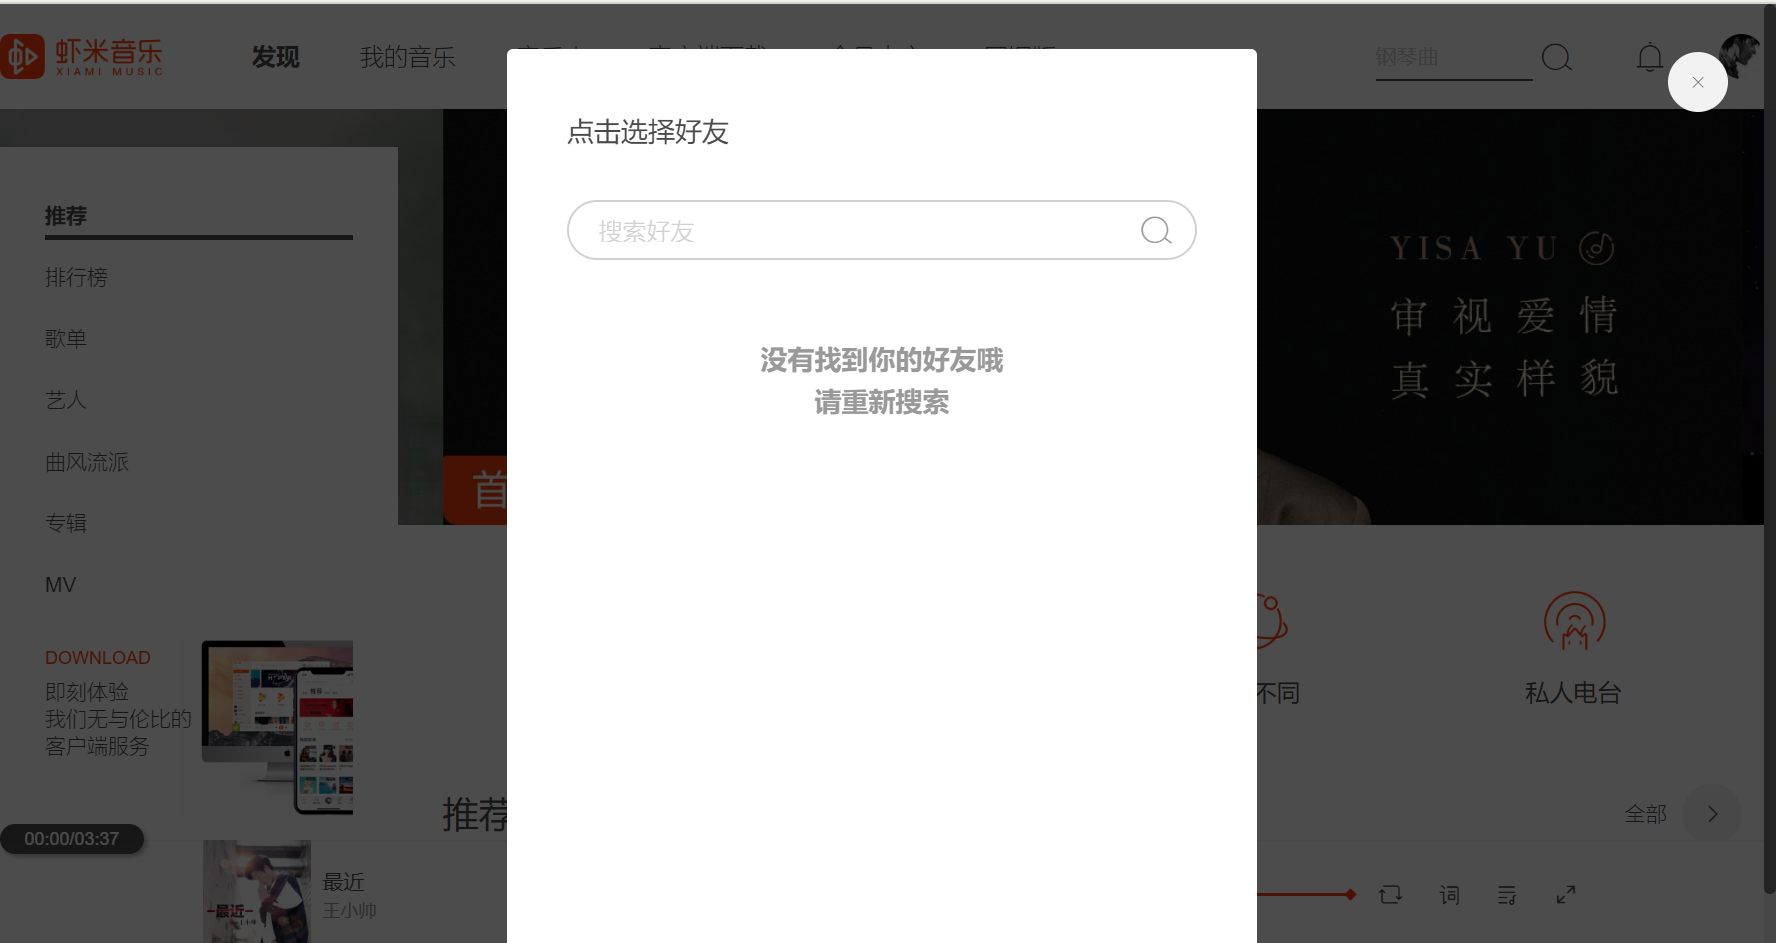
\includegraphics[width=0.5\textwidth]{./figures/capture6.png} 
	
		\end{center}
   输入:用户通过鼠标点选其中一个类型及其类别。
   
   
   \subsubsection{处理}
   
   
   
   A. 输入数据的有效性检测:不需要进行有效性检测,因为输入是通过鼠标在对应区域点击引起中断造成的。
   
   B. 操作的确切次序:
   \begin{adjustwidth}{2cm}{1cm}\qquad
	   \begin{itemize}
		   \item 中断事件发生
		   \item 调用监听函数
		   \item 客户端向服务器请求用户表单,服务器通过查询数据库得到相应表单回送到客户端
		   \item 网页重定向到分享页面
		   \item 用户选择想要分享的用户账户,点击确认
		   \item 客户端向数据库发送分享请求,并传输必要的数据(如专辑/歌单/单曲的id)
		   \item 数据库接收到分享请求,在分享表单里添加对应表项;并设置用户表单中,被分享用户的未读消息属性为1;
		   \item 数据库向客户端回送成功消息
		   \item 监听函数接收到成功消息
		   \item 刷新网页,将数据以合适的方式显示给用户
	   \end{itemize}		
   \end{adjustwidth}
	
   
   C. 对异常情况的回应,例如:
   \begin{adjustwidth}{2cm}{1cm}\qquad
	   \begin{itemize}
		   \item 溢出
		   \item 通信失败
		   \item 错误处理
	   \end{itemize}		
   \end{adjustwidth}
   
	   发生以上错误时,函数体向网页返回错误代码,网页打印相应错误信息
   
D. 通过过程性sql指令向数据库传送查询请求
		   
   E. 对输出数据的有效性检测:
   
   在监听函数接收到数据库传送过来的数据后,首先进行合法性检测,如果合法则令网页正常显示;如果数据不合法或不安全——返回错误代码,让网页打印错误信息;
   
   \subsubsection{输出}
   
   A. 输出描述:
   \begin{itemize}
	\item	输出:动态网页显示
	\item	数量:1
	\item	度量单位:页
	\item	时序:无
	\item	包含精确度和容忍度的有效输出范围:无
	\item	对非法值的处理:打印错误信息
	\item	错误消息:当输出不合法时,打印网页不存在或者输入信息错误;
   \end{itemize}
   详细描述:
   数据库中增加分享表单条目,并回送对应消息到网页,表示分享已经成功
 




   \subsection{URS\_Look-up\_F04 查看分享}

   \subsubsection{介绍}
   
   用户登录,并跳转到分享消息页面
   
   错误输入:因为是鼠标点击输入,所以不存在错误输入
   
   非法条件:没有登录,直接点击分享
   
   无效输入:无
   \begin{center} 
	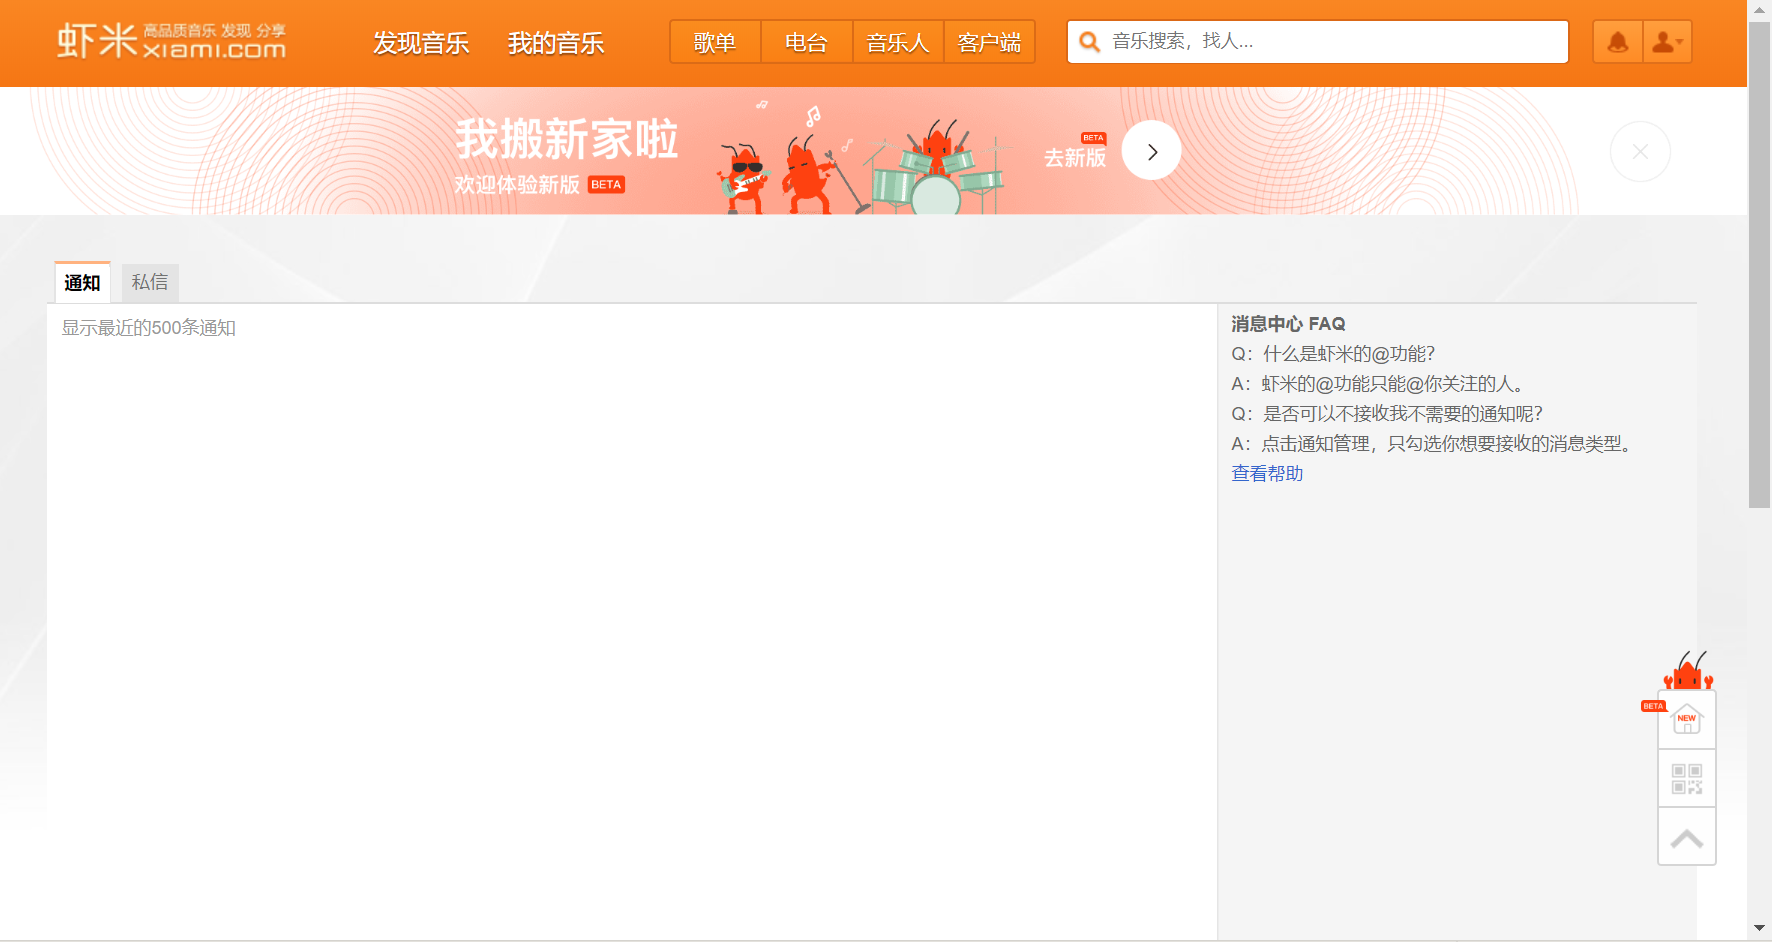
\includegraphics[width=0.5\textwidth]{./figures/capture7.png} 

	\end{center}
   \subsubsection{输入}
   
   输入:用户通过鼠标点选其中一个类型及其类别。
   
   
   \subsubsection{处理}
   
   
   
   A. 输入数据的有效性检测:不需要进行有效性检测,因为输入是通过鼠标在对应区域点击引起中断造成的。
   
   B. 操作的确切次序:
   \begin{adjustwidth}{2cm}{1cm}\qquad
	   \begin{itemize}
		   \item 中断事件发生
		   \item 调用监听函数
		   \item 客户端向服务器请求分享表单,服务器通过查询数据库得到相应表单回送到客户端
		   \item 将相应条目显示到网页上
		   \item 如果用户点击分享相应条目,则客户端向服务器发送查询请求
		   \item 服务器数据库回送相应的资源的url
		   \item 客户端解析相应url,并重定向为歌单/专辑/单曲页面
		   \item 监听函数接收到成功消息
		   \item 刷新网页,将数据以合适的方式显示给用户
	   \end{itemize}		
   \end{adjustwidth}
	
   
   C. 对异常情况的回应,例如:
   \begin{adjustwidth}{2cm}{1cm}\qquad
	   \begin{itemize}
		   \item 溢出
		   \item 通信失败
		   \item 错误处理
	   \end{itemize}		
   \end{adjustwidth}
   
	   发生以上错误时,函数体向网页返回错误代码,网页打印相应错误信息
   
D. 通过过程性sql指令向数据库传送查询请求
		   
   E. 对输出数据的有效性检测:
   
   在监听函数接收到数据库传送过来的数据后,首先进行合法性检测,如果合法则令网页正常显示;如果数据不合法或不安全——返回错误代码,让网页打印错误信息;
   
   \subsubsection{输出}
   
   A. 输出描述:
   \begin{itemize}
	\item	输出:动态网页播放
	\item	数量:1
	\item	度量单位:页
	\item	时序:无
	\item	包含精确度和容忍度的有效输出范围:无
	\item	对非法值的处理:打印错误信息
	\item	错误消息:当输出不合法时,打印网页不存在或者输入信息错误;
   \end{itemize}
   详细描述:
   回送分享条目所对应url,解析并渲染,输出为网页


   \subsection{URS\_Mark\_F05评分}

   \subsubsection{介绍}
   
   用户需要点击播放栏的“最大化”按键,跳转到播放页面,然后点击评分按键
   
   错误输入:因为是鼠标点击输入,所以不存在错误输入
   
   非法条件:没有登录,直接点击分享
   
   无效输入:无
   \begin{center} 
	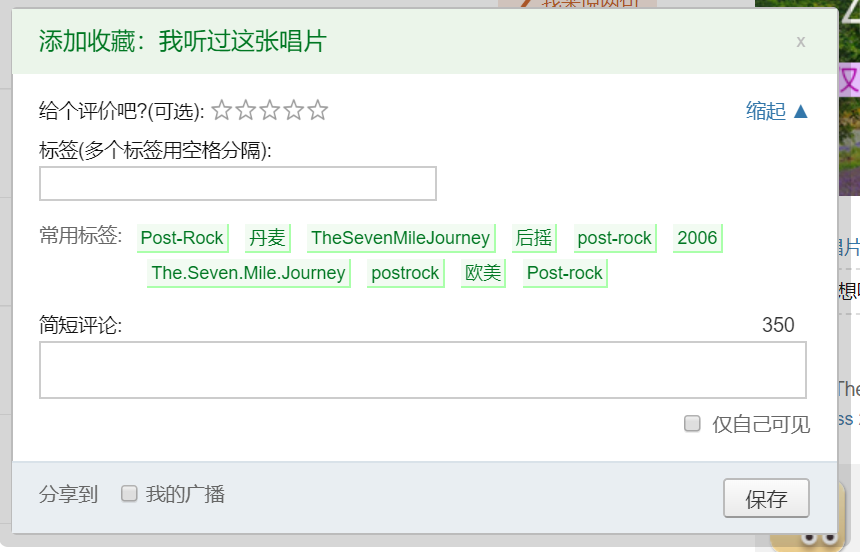
\includegraphics[width=0.7\textwidth]{./figures/capture8.png} 
	\end{center}
   
   输入:用户通过鼠标点选其中一个类型及其类别。
   
   
   \subsubsection{处理}
   
   
   
   A. 输入数据的有效性检测:不需要进行有效性检测,因为输入是通过鼠标在对应区域点击引起中断造成的。
   
   B. 操作的确切次序:
   \begin{adjustwidth}{2cm}{1cm}\qquad
	   \begin{itemize}
		\item 中断事件发生
		\item 调用监听函数
		\item 客户端重定向到评分页面
		\item 用户输入一个一到十以内的数字,并点击“确认”
		\item 客户端向数据库发送评分请求
		\item 数据库在评分表单里增加相应条目,更新相应音乐的评分属性,并回送成功消息
		\item 客户端打印成功消息
	   \end{itemize}		
   \end{adjustwidth}
	
   
   C. 对异常情况的回应,例如:
   \begin{adjustwidth}{2cm}{1cm}\qquad
	   \begin{itemize}
		   \item 溢出
		   \item 通信失败
		   \item 错误处理
	   \end{itemize}		
   \end{adjustwidth}
   
	   发生以上错误时,函数体向网页返回错误代码,网页打印相应错误信息
   
D. 通过过程性sql指令向数据库传送查询请求
		   
   E. 对输出数据的有效性检测:
   
   在监听函数接收到数据库传送过来的数据后,首先进行合法性检测,如果合法则令网页正常显示;如果数据不合法或不安全——返回错误代码,让网页打印错误信息;
   
   \subsubsection{输出}
   
   A. 输出描述:
   \begin{itemize}
	\item	输出:动态网页播放
	\item	数量:1
	\item	度量单位:页
	\item	时序:无
	\item	包含精确度和容忍度的有效输出范围:无
	\item	对非法值的处理:打印错误信息
	\item	错误消息:当输出不合法时,打印网页不存在或者输入信息错误;
   \end{itemize}
   详细描述:更新服务器中的用户评分历史记录,修改对应音乐的平均分;回送成功消息到网页


   \subsection{URS\_Charts\_F06 排行榜}

   \subsubsection{介绍}
   
   用户登录,并跳转到排行榜页面
   
   错误输入:因为是鼠标点击输入,所以不存在错误输入
   
   非法条件:没有登录,直接点击分享
   
   无效输入:无
   \begin{center} 
	\begin{sideways}
	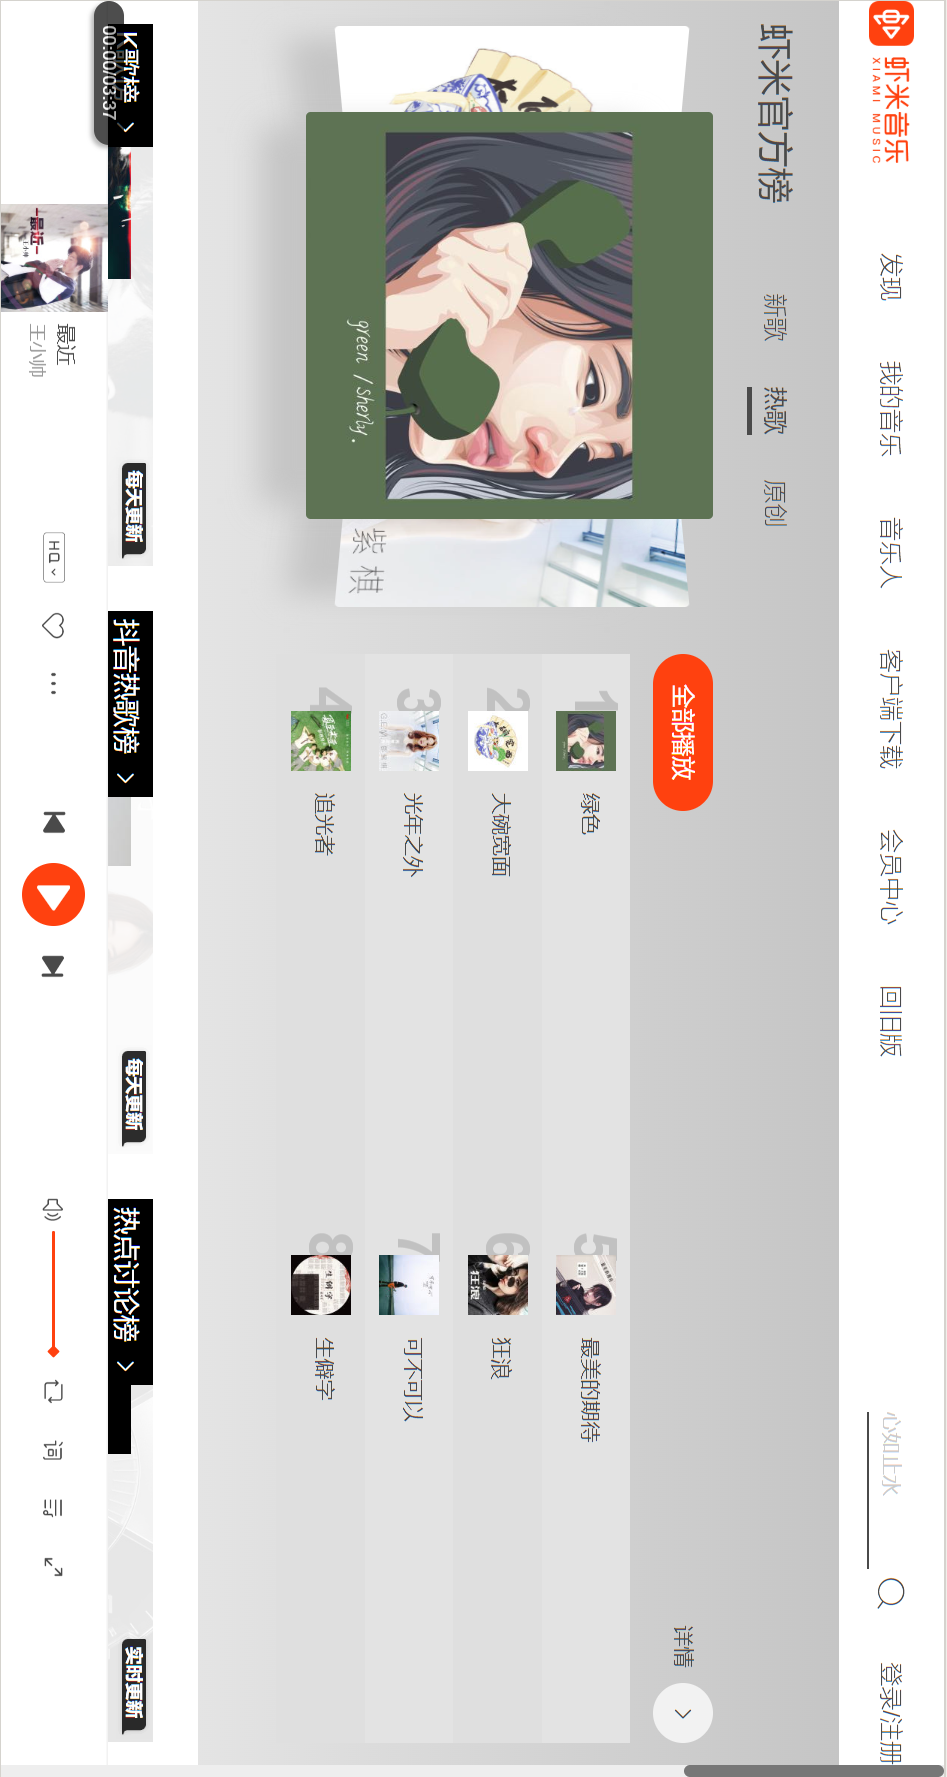
\includegraphics[width=0.5\textwidth]{./figures/capture9.png} 
	\end{sideways}
	\end{center}
   \subsubsection{输入}
   
   输入:用户通过鼠标点选其中一个类型及其类别。
   
   
   \subsubsection{处理}
   
   
   
   A. 输入数据的有效性检测:不需要进行有效性检测,因为输入是通过鼠标在对应区域点击引起中断造成的。
   
   B. 操作的确切次序:
   \begin{adjustwidth}{2cm}{1cm}\qquad
	   \begin{itemize}
		\item 中断事件发生
		\item 调用监听函数
		\item 客户端向服务器发送排行榜请求
		\item 服务器在数据库中查询排行榜表单
		\item 另外,服务器将排行榜中的第一首可播放歌曲文件也传输到客户端
		\item 监听器感知到回送数据,刷新网页,网页播放歌单中的第一首歌曲
		\item 如果用户在推荐页面切换歌曲,则客户端向查询本地的排行榜表单信息,向服务器请求本地歌单中的下一首歌
	   \end{itemize}		
   \end{adjustwidth}
	
   
   C. 对异常情况的回应,例如:
   \begin{adjustwidth}{2cm}{1cm}\qquad
	   \begin{itemize}
		   \item 溢出
		   \item 通信失败
		   \item 错误处理
	   \end{itemize}		
   \end{adjustwidth}
   
	   发生以上错误时,函数体向网页返回错误代码,网页打印相应错误信息
   
D. 通过过程性sql指令向数据库传送查询请求
		   
   E. 对输出数据的有效性检测:
   
   在监听函数接收到数据库传送过来的数据后,首先进行合法性检测,如果合法则令网页正常显示;如果数据不合法或不安全——返回错误代码,让网页打印错误信息;
   
   \subsubsection{输出}
   
   A. 输出描述:
   \begin{itemize}
	\item	输出:动态网页播放
	\item	数量:1
	\item	度量单位:页
	\item	时序:无
	\item	包含精确度和容忍度的有效输出范围:无
	\item	对非法值的处理:打印错误信息
	\item	错误消息:当输出不合法时,打印网页不存在或者输入信息错误;
   \end{itemize}
   详细描述:回送排行榜信息,以及第一首可播放曲目文件到客户端







   \subsection{URS\_Reco-Songs\_F07 推荐歌曲}

   \subsubsection{介绍}
   % \iffalse
   
   % 逐条列出与本特性相关的功能需求。包括项目如何响应预期的错误输入,非法条件和无效输入。需求应该简明,完整,不含糊,可验证,必要的。 当需要的信息不确定的时候使用“待定”。
   % \fi
   本部分应用程序的目的是使客户能够找到他所选歌曲的推荐。
   \begin{center} 
	\begin{sideways}
	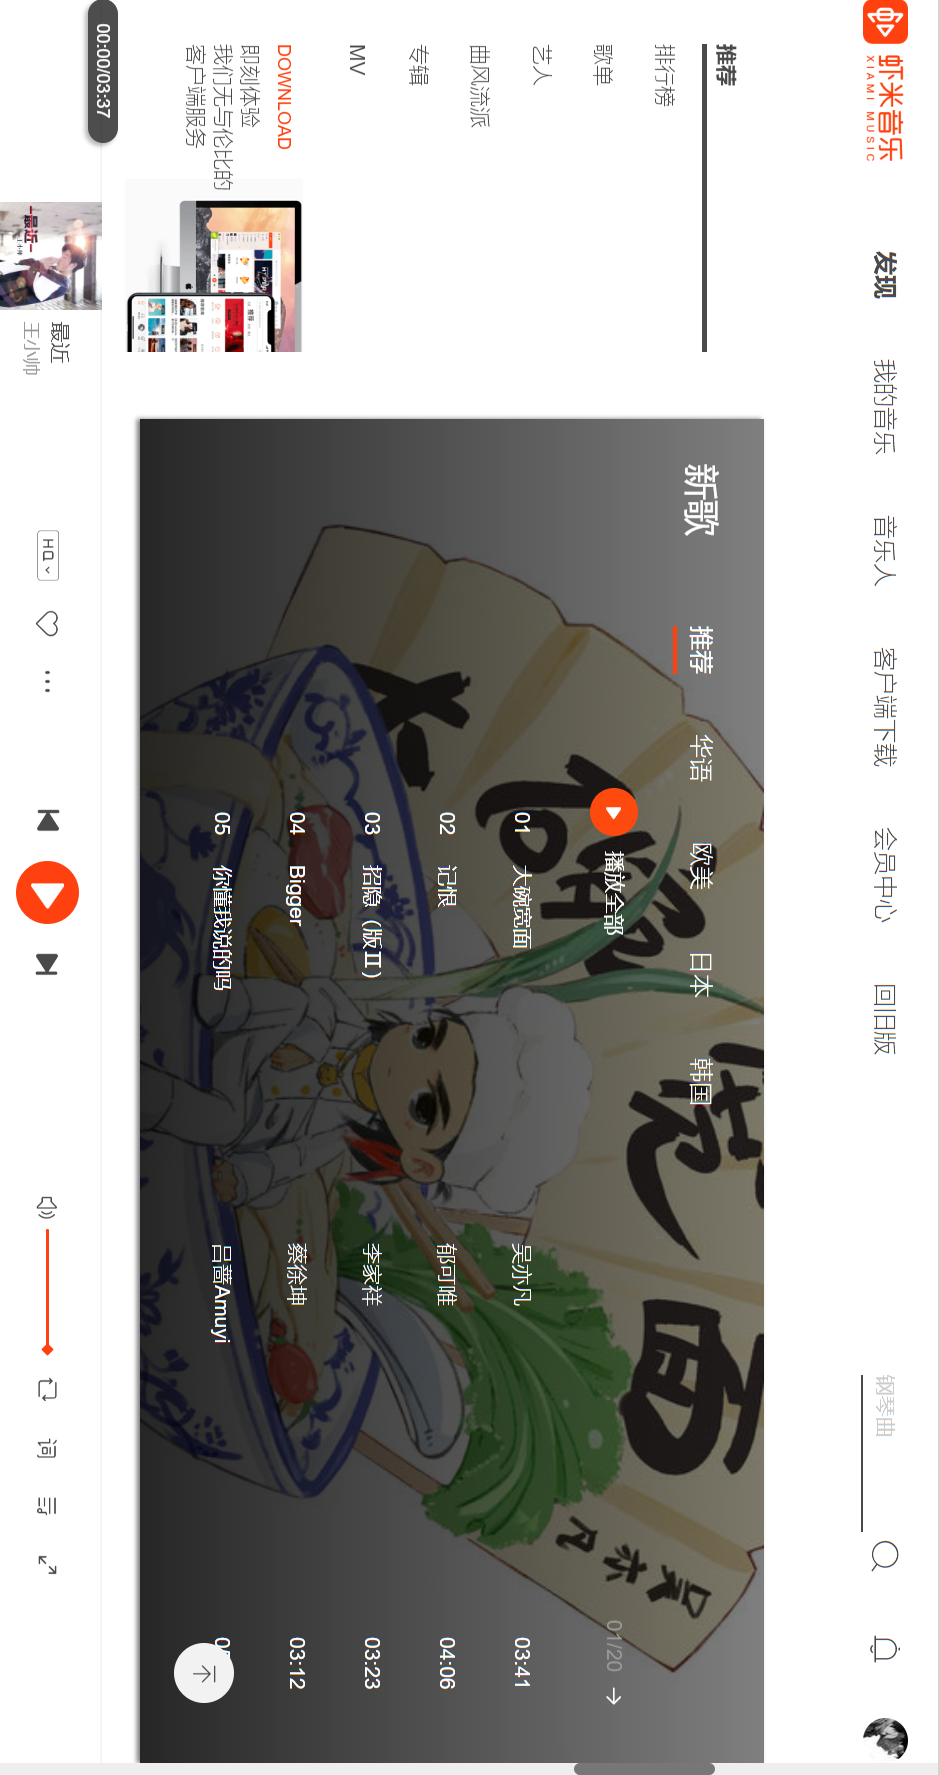
\includegraphics[width=0.5\textwidth]{./figures/capture10.png} 
	\end{sideways}
	\end{center}
   \subsubsection{输入}
   
   输入:用户在登录默认页面,点击“推荐”,即进入推荐页面
   
   \subsubsection{处理}
   

   
   A. 输入数据的有效性检测:不需要进行有效性检测,因为输入是通过鼠标在对应区域点击引起中断造成的。
   
   B. 操作的确切次序:
   \begin{adjustwidth}{2cm}{1cm}\qquad
	   \begin{itemize}
		   \item 中断事件发生
		   \item 调用监听函数
		   \item 客户端向服务器发送推荐请求
		   \item 服务器首先在数据库中查询用户的歌曲评分历史记录
		   \item 如果历史记录为空,则将排行榜歌单信息回送到客户端;如果评分历史记录不为空,则调用相应的推荐算法,回送推荐算法输出的歌单信息到数据库。
		   \item 另外,服务器将推荐歌单中的第一首可播放歌曲文件也传输到客户端
		   \item 监听器感知到回送数据,刷新网页,网页播放歌单中的第一首歌曲
		   \item 如果用户在推荐页面切换歌曲,则客户端向查询本地的推荐歌单信息,向服务器请求本地歌单中的下一首歌
	   \end{itemize}		
   \end{adjustwidth}
	
   
   C. 对异常情况的回应,例如:
   \begin{adjustwidth}{2cm}{1cm}\qquad
	   \begin{itemize}
		   \item 溢出
		   \item 通信失败
		   \item 错误处理
	   \end{itemize}		
   \end{adjustwidth}
   
	   发生以上错误时,函数体向网页返回错误代码,网页打印相应错误信息
   D.通过特定数据结构发送服务器可识别的推荐请求
		   
   E. 对输出数据的有效性检测:
   
   在监听函数接收到数据库传送过来的数据后,首先进行合法性检测,如果合法则令网页正常显示;如果数据不合法或不安全——返回错误代码,让网页打印错误信息;
   
   \subsubsection{输出}
   \begin{itemize}
	   \item	输出:动态网页播放
	   \item	数量:1
	   \item	度量单位:页
	   \item	时序:无
	   \item	包含精确度和容忍度的有效输出范围:无
	   \item	对非法值的处理:打印错误信息
	   \item	错误消息:当输出不合法时,打印网页不存在或者输入信息错误;
	  \end{itemize}
	  详细描述:通过考察用户历史评分记录,根据推荐算法得出用户最可能喜欢的歌曲集,回送歌单信息,以及第一首可播放曲目到客户端






	  \subsection{URS\_Login\_F08 账户登陆}
	
	  \subsubsection{介绍}
	  该功能的目的是完成用户认证,每一个实际存在的用户都应该有一个有效的账户。
	  \begin{center} 
		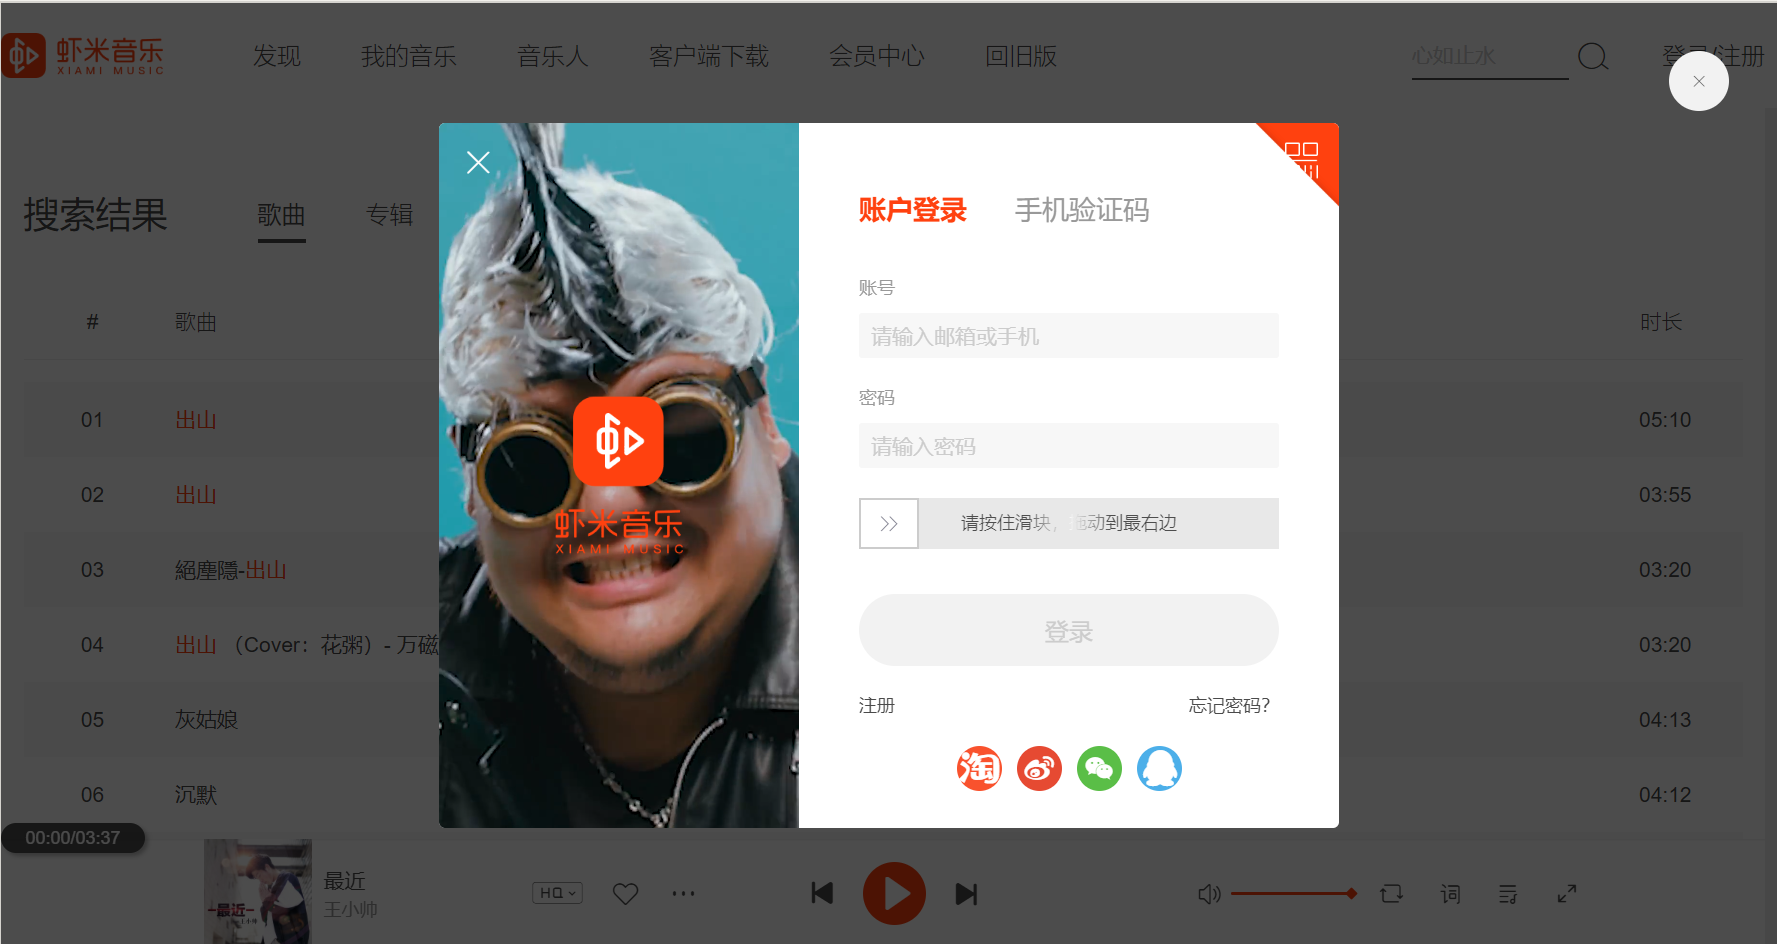
\includegraphics[width=0.8\textwidth]{./figures/capture4.png} 
		\end{center}
	  \subsubsection{输入}
	  
	  输入:客户可以通过输入用户名和密码登录音乐商城。
	  
	  \subsubsection{处理}
	  
	  
	  
	  A. 输入数据的有效性检测:不需要进行有效性检测,因为输入是通过鼠标在对应区域点击引起中断造成的。
	  
	  B. 操作的确切次序:
	  \begin{adjustwidth}{2cm}{1cm}\qquad
		  \begin{itemize}
			  \item 中断事件发生
			  \item 调用监听函数
			  \item 用户可以输入账户和密码
			  \item 文本输入完毕后,单击“Login”按钮
			  \item 将输入文本转化为数据库查询,传送到服务器端
			  \item 服务器验证用户名和密码是否匹配,然后根据匹配结果回送数据到客户端
			  \item 监听器感知到回送数据,刷新网页
		  \end{itemize}		
	  \end{adjustwidth}
	   
	  
	  C. 对异常情况的回应,例如:
	  \begin{adjustwidth}{2cm}{1cm}\qquad
		  \begin{itemize}
			  \item 溢出
			  \item 通信失败
			  \item 错误处理
		  \end{itemize}		
	  \end{adjustwidth}
	  
		  发生以上错误时,函数体向网页返回错误代码,网页打印相应错误信息
	  D. 通过tcp协议向服务器传输有关数据
			  
	  E. 对输出数据的有效性检测:
	  
	  在监听函数接收到数据库传送过来的数据后,首先进行合法性检测,如果合法则令网页正常显示;如果数据不合法或不安全——返回错误代码,让网页打印错误信息;
	  
	  \subsubsection{输出}
	  \begin{itemize}
		  \item	输出:动态网页显示
		  \item	数量:1
		  \item	度量单位:页
		  \item	时序:无
		  \item	包含精确度和容忍度的有效输出范围:无
		  \item	对非法值的处理:打印错误信息
		  \item	错误消息:当输出不合法时,打印网页不存在或者输入信息错误;
		 \end{itemize}
		 详细描述:系统将验证登录名是否与登录密码匹配:
		 如果用户名或密码无效,将在页面上打印相应的错误消息,并要求用户重新输入用户名和密码。
		 如果用户输入有效,将显示主页面。






		 \subsection{URS\_Register\_F09 账户注册}

		 \subsubsection{介绍}
		 该功能的目的是使得新用户能够进行注册;必须为现有用户保留有效的账号,否则新用户的注册会覆盖已有用户。
		 \begin{center} 
			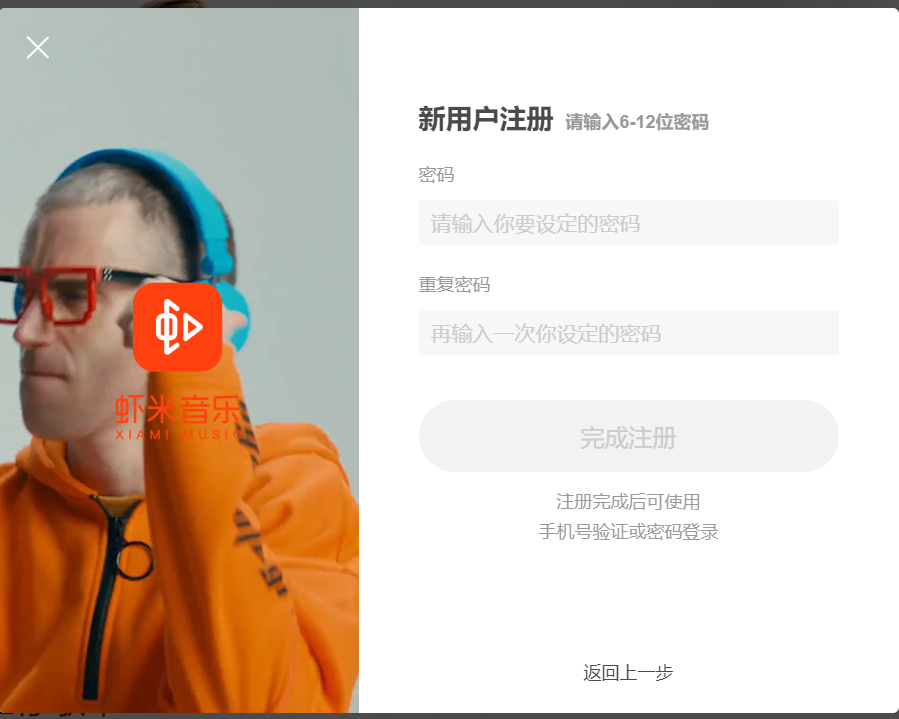
\includegraphics[width=0.8\textwidth]{./figures/capture11.png} 
			\end{center}
		 \subsubsection{输入}
		 
		 输入:如果客户是新用户,他可以请求在系统中进行注册。
		 
		 \subsubsection{处理}
		 
		 
		 
		 A. 输入数据的有效性检测:不需要进行有效性检测,因为输入是通过鼠标在对应区域点击引起中断造成的。
		 
		 B. 操作的确切次序:
		 \begin{adjustwidth}{2cm}{1cm}\qquad
			 \begin{itemize}
				 \item 中断事件发生
				 \item 调用监听函数
				 \item 重定向到注册页面
				 \item 用户选择用户名,密码并输入有效的电子邮件ID,安全问题和答案
				 \item 文本输入完毕后,单击“Sign Up”按钮
				 \item 将输入文本转化为数据库查询,传送到服务器端
				 \item 服务器检查用户输入是否合法:如果合法,在用户档案数据库中增加新表项,并返回注册成功信息;
				 \item 否则,回送错误代码
				 \item 监听器感知到回送数据,刷新网页
			 \end{itemize}		
		 \end{adjustwidth}
		  
		 
		 C. 对异常情况的回应,例如:
		 \begin{adjustwidth}{2cm}{1cm}\qquad
			 \begin{itemize}
				 \item 溢出
				 \item 通信失败
				 \item 错误处理
			 \end{itemize}		
		 \end{adjustwidth}
		 
			 发生以上错误时,函数体向网页返回错误代码,网页打印相应错误信息
		 D. 通过tcp协议向服务器传输有关数据
				 
		 E. 对输出数据的有效性检测:
		 
		 在监听函数接收到数据库传送过来的数据后,首先进行合法性检测,如果合法则令网页正常显示;如果数据不合法或不安全——返回错误代码,让网页打印错误信息;
		 
		 \subsubsection{输出}
		 \begin{itemize}
			 \item	输出:动态网页显示
			 \item	数量:1
			 \item	度量单位:页
			 \item	时序:无
			 \item	包含精确度和容忍度的有效输出范围:无
			 \item	对非法值的处理:打印错误信息
			 \item	错误消息:当输出不合法时,打印网页不存在或者输入信息错误;
			\end{itemize}
			详细描述:如果成功,显示注册成功页面。如果注册不成功,显示注册失败页面并打印失败原因。






			\subsection{URS\_Logout\_F010 账户注销}

			\subsubsection{介绍}
			该功能的目的是完成用户注销,退出登录。
			\subsubsection{输入}
			
			输入:已登录用户可以通过点击注销按钮完成注销。
			
			\subsubsection{处理}
			
			
			
			A. 输入数据的有效性检测:不需要进行有效性检测,因为输入是通过鼠标在对应区域点击引起中断造成的。
			
			B. 操作的确切次序:
			\begin{adjustwidth}{2cm}{1cm}\qquad
				\begin{itemize}
					\item 中断事件发生
					\item 调用监听函数
					\item 用户单击“Logout”按钮
					\item 将输入文本转化为数据库查询,传送到服务器端
					\item 服务器修改数据库中用户表的登录信息属性,将结果回送数据到客户端
					\item 监听器感知到回送数据,刷新网页
				\end{itemize}		
			\end{adjustwidth}
			 
			
			C. 对异常情况的回应,例如:
			\begin{adjustwidth}{2cm}{1cm}\qquad
				\begin{itemize}
					\item 溢出
					\item 通信失败
					\item 错误处理
				\end{itemize}		
			\end{adjustwidth}
			
				发生以上错误时,函数体向网页返回错误代码,网页打印相应错误信息
			D. 通过tcp协议向服务器传输有关数据
					
			E. 对输出数据的有效性检测:
			
			在监听函数接收到数据库传送过来的数据后,首先进行合法性检测,如果合法则令网页正常显示;如果数据不合法或不安全——返回错误代码,让网页打印错误信息;
			
			\subsubsection{输出}
			\begin{itemize}
				\item	输出:动态网页显示
				\item	数量:1
				\item	度量单位:页
				\item	时序:无
				\item	包含精确度和容忍度的有效输出范围:无
				\item	对非法值的处理:打印错误信息
				\item	错误消息:当输出不合法时,打印网页不存在或者输入信息错误;
			   \end{itemize}
			   详细描述:系统根据用户传来的ID修改数据库中对应元组的登录属性,成功修改以后,显示登录界面。

			
			   \subsubsection{介绍:绑定信用卡}
			   该功能的目的是完成用户信用卡的绑定,一个用户可以绑定一张信用卡。
			   \begin{center} 
				 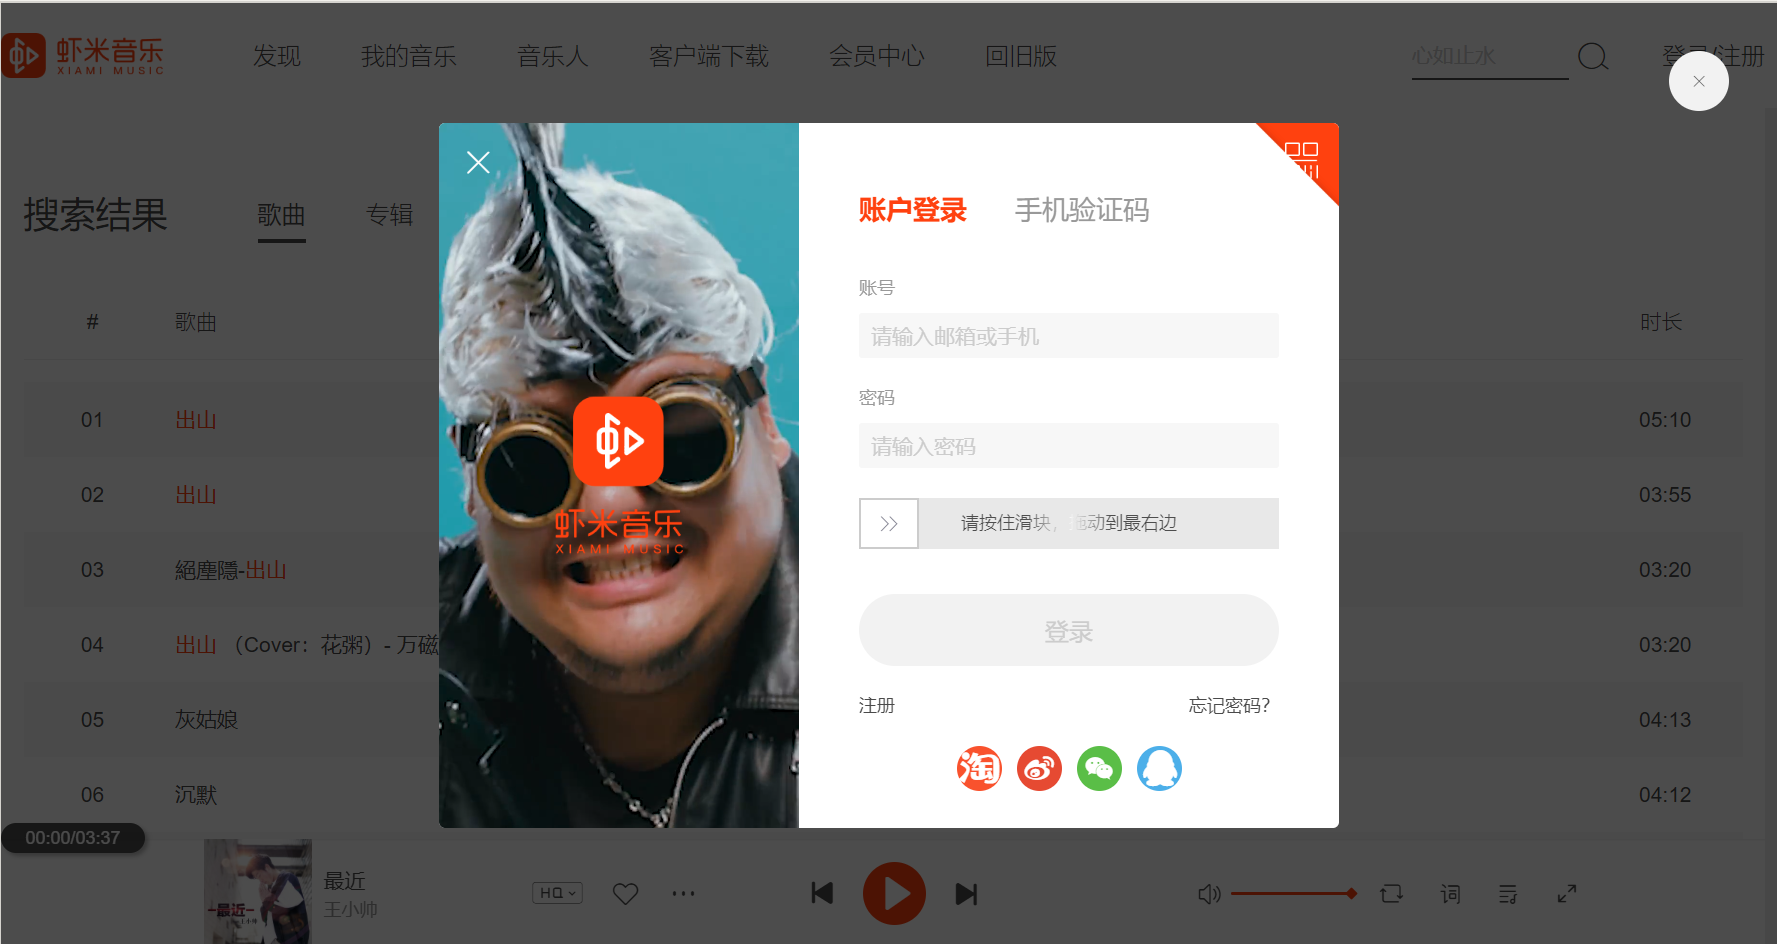
\includegraphics[width=0.8\textwidth]{./figures/capture4.png} 
				 \end{center}
			   \subsubsection{输入}
			   
			   输入:客户可以在账户编辑页面通过输入银行卡号来绑定银行卡。
			   
			   \subsubsection{处理}
			   
			   
			   
			   A. 输入数据的有效性检测:输入的银行卡号必须是由16个0~9的整数组成的字符串,否则不合法。监听函数将根据这个标准进行合法性检测。
			   
			   B. 操作的确切次序:
			   \begin{adjustwidth}{2cm}{1cm}\qquad
				   \begin{itemize}
					   \item 中断事件发生
					   \item 调用监听函数
					   \item 用户可以银行卡号,
					   \item 文本输入完毕后,单击“绑定”按钮
					   \item 将输入文本转化为数据库查询,传送到服务器端
					   \item 服务器更新数据库中对应用户的信用卡号属性
					   \item 监听器感知到回送数据,刷新网页
				   \end{itemize}		
			   \end{adjustwidth}
				
			   
			   C. 对异常情况的回应,例如:
			   \begin{adjustwidth}{2cm}{1cm}\qquad
				   \begin{itemize}
					   \item 溢出
					   \item 通信失败
					   \item 错误处理
				   \end{itemize}		
			   \end{adjustwidth}
			   
				   发生以上错误时,函数体向网页返回错误代码,网页打印相应错误信息
			   D. 通过tcp协议向服务器传输有关数据
					   
			   E. 对输出数据的有效性检测:
			   
			   在监听函数接收到数据库传送过来的数据后,首先进行合法性检测,如果合法则令网页正常显示;如果数据不合法或不安全——返回错误代码,让网页打印错误信息;
			   
			   \subsubsection{输出}
			   \begin{itemize}
				   \item	输出:动态网页显示
				   \item	数量:1
				   \item	度量单位:页
				   \item	时序:无
				   \item	包含精确度和容忍度的有效输出范围:无
				   \item	对非法值的处理:打印错误信息
				   \item	错误消息:当输出不合法时,打印网页不存在或者输入信息错误;
				  \end{itemize}
				  详细描述:系统将更新用户的信用卡号信息。如果用户输入了合法的信用卡号,显示绑定成功的消息,否则显示绑定失败并提示失败原因。
		 

\subsection{URS\_Order\_F011 将歌曲加入购物车}

   \subsubsection{介绍}
   实现在搜索或浏览目录时将产品添加到购物车。
   前提条件:用户必须登录才能将商品(单曲或者专辑)添加到购物车,使用insert命令将商品添加到数据库中的购物车表中
   \begin{center}
	\begin{sideways} 
   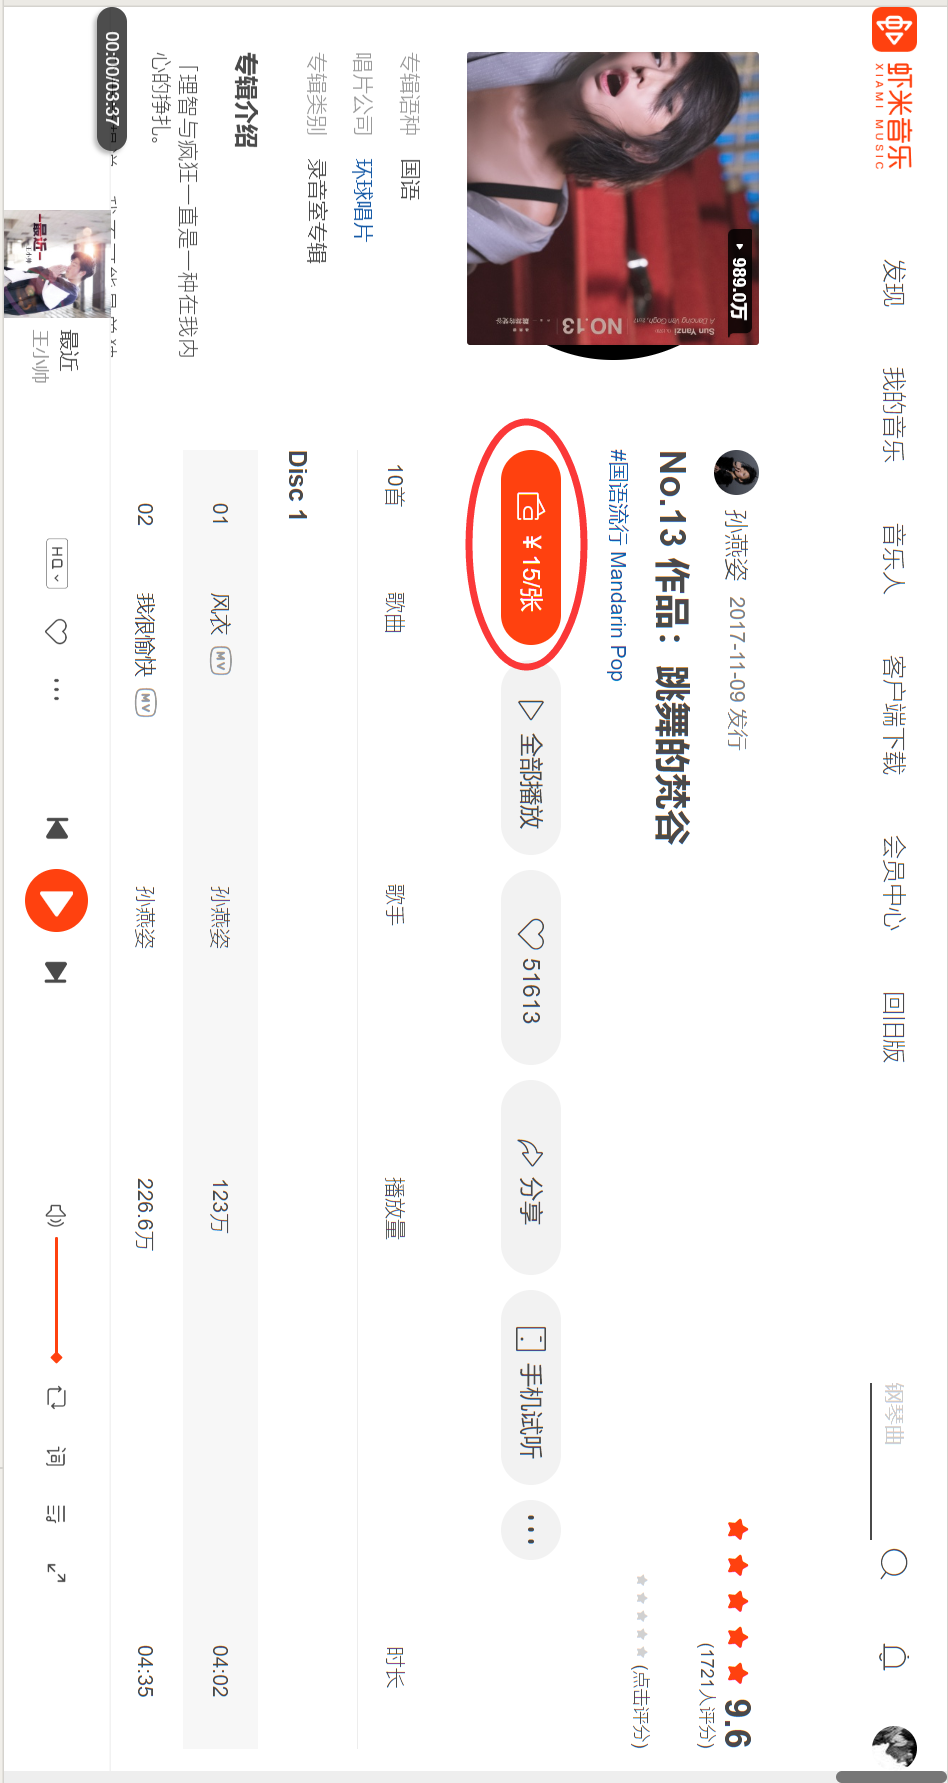
\includegraphics[width=0.5\textwidth]{./figures/capture12.png} 
	\end{sideways}
\end{center}
   \subsubsection{输入}
   
   当用户找到他想要的产品时,用户通过点击“添加到购物车”按钮将它们添加到购物车


   \subsubsection{处理}
   

   
   A. 输入数据的有效性检测:不需要进行有效性检测,因为输入是通过鼠标在对应区域点击引起中断造成的。
   
   B. 操作的确切次序:
   \begin{adjustwidth}{2cm}{1cm}\qquad
	   \begin{itemize}
		   \item 中断事件发生
		   \item 调用监听函数
		   \item 将数据库插入请求传送到服务器端
		   \item 服务器回送传输成功信息到客户端
		   \item 监听器感知到回送数据,刷新网页
	   \end{itemize}		
   \end{adjustwidth}
	
   
   C. 对异常情况的回应,例如:
   \begin{adjustwidth}{2cm}{1cm}\qquad
	   \begin{itemize}
		   \item 溢出
		   \item 通信失败
		   \item 错误处理
	   \end{itemize}		
   \end{adjustwidth}
   
	   发生以上错误时,函数体向网页返回错误代码,网页打印相应错误信息
   
D. 通过过程性sql指令向数据库传送查询请求
		   
   E. 对输出数据的有效性检测:
   
   在监听函数接收到数据库传送过来的数据后,首先进行合法性检测,如果合法则令网页正常显示;如果数据不合法或不安全——返回错误代码,让网页打印错误信息;
   
   \subsubsection{输出}
   \begin{itemize}
	   \item	输出:用户档案数据库增加一个表项
	   \item	数量:1
	   \item	度量单位:条
	   \item	时序:无
	   \item	包含精确度和容忍度的有效输出范围:无
	   \item	对非法值的处理:打印错误信息
	   \item	错误消息:当输出不合法时,打印网页不存在或者输入信息错误;
	  \end{itemize}
	  详细描述:产品将被添加到购物车中,用户档案数据库中增加相应条目。






	  \subsection{URS\_Look-cart\_F012 查看购物车}
   \subsubsection{介绍}
   在搜索或浏览目录时查看购物车的内容,将使用选择查询显示购物车表的内容。
   前提条件:用户必须登录并且购物车必须至少有一个条目才能查看购物车的详细信息。
   \begin{center}
	\begin{sideways} 
   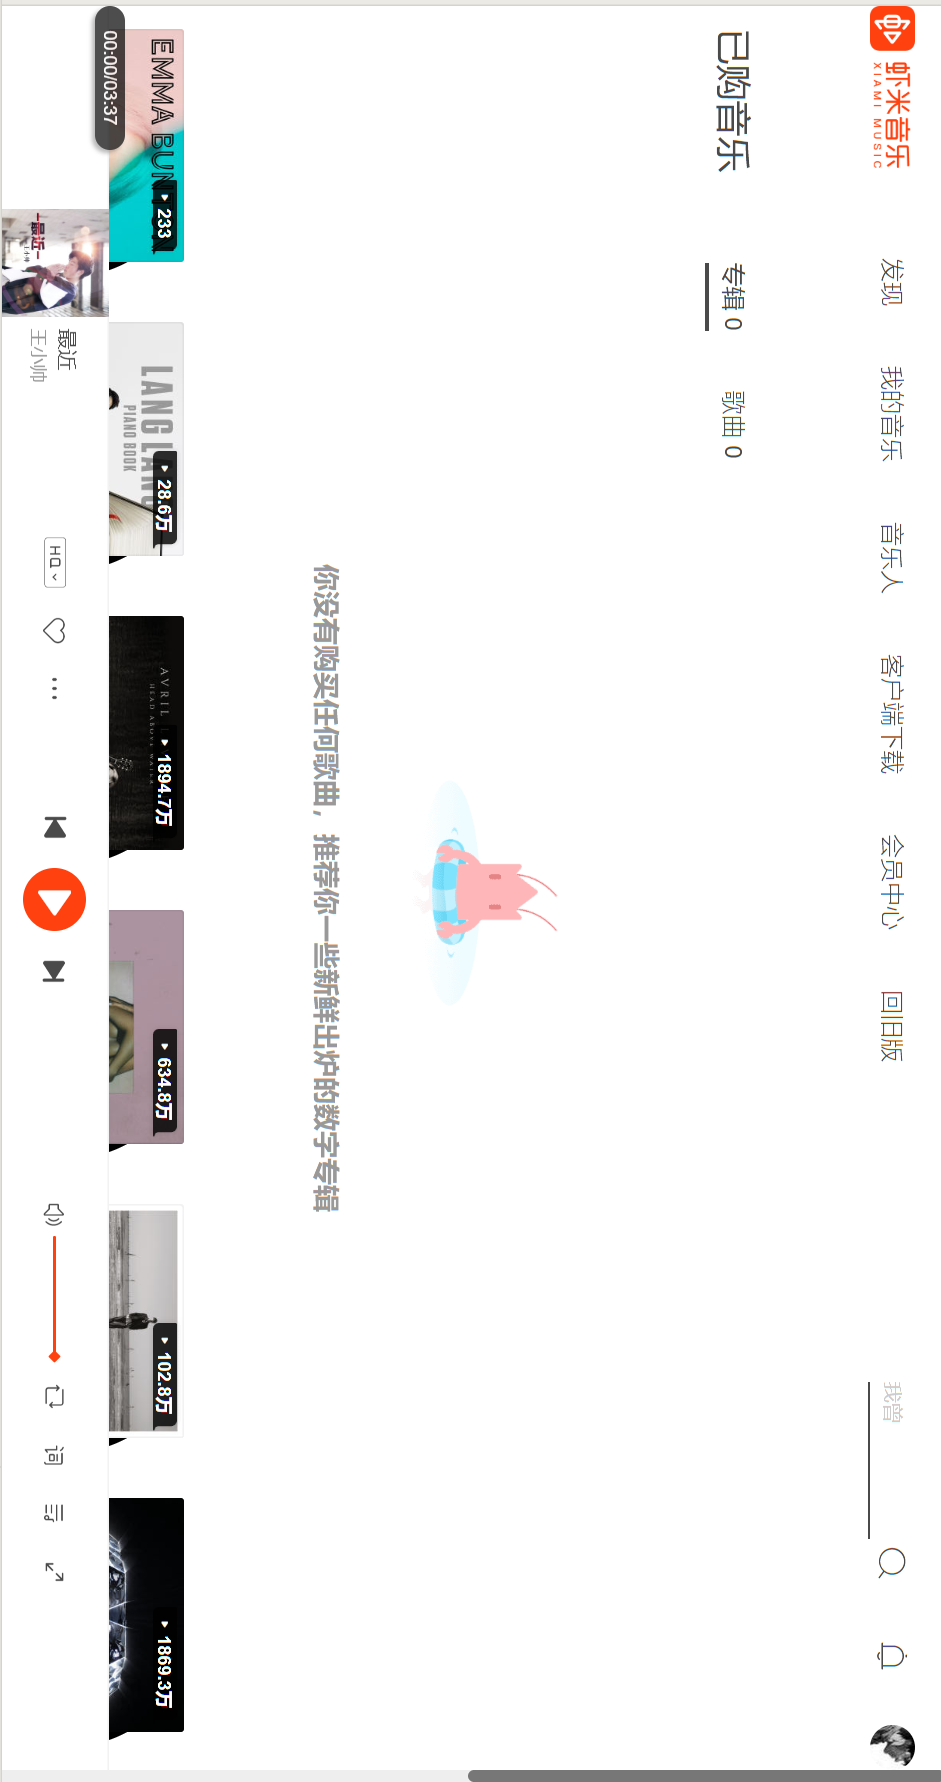
\includegraphics[width=0.5\textwidth]{./figures/capture13.png} 
	\end{sideways}
\end{center}
   \subsubsection{输入}
   
   客户可以通过单击“查看详细信息”按钮请求查看购物车的内容。


   \subsubsection{处理}
   

   
   A. 输入数据的有效性检测:不需要进行有效性检测,因为输入是通过鼠标在对应区域点击引起中断造成的。
   
   B. 操作的确切次序:
   \begin{adjustwidth}{2cm}{1cm}\qquad
	   \begin{itemize}
		   \item 中断事件发生
		   \item 调用监听函数
		   \item 将数据库查询请求传送到服务器端
		   \item 服务器回送相关数据到客户端
		   \item 监听器感知到回送数据,刷新网页
	   \end{itemize}		
   \end{adjustwidth}
	
   
   C. 对异常情况的回应,例如:
   \begin{adjustwidth}{2cm}{1cm}\qquad
	   \begin{itemize}
		   \item 溢出
		   \item 通信失败
		   \item 错误处理
	   \end{itemize}		
   \end{adjustwidth}
   
	   发生以上错误时,函数体向网页返回错误代码,网页打印相应错误信息
   
D. 通过过程性sql指令向数据库传送查询请求
		   
   E. 对输出数据的有效性检测:
   
   在监听函数接收到数据库传送过来的数据后,首先进行合法性检测,如果合法则令网页正常显示;如果数据不合法或不安全——返回错误代码,让网页打印错误信息;
   
   \subsubsection{输出}
   \begin{itemize}
	   \item	输出:用户档案数据库增加一个表项
	   \item	数量:1
	   \item	度量单位:条
	   \item	时序:无
	   \item	包含精确度和容忍度的有效输出范围:无
	   \item	对非法值的处理:打印错误信息
	   \item	错误消息:当输出不合法时,打印网页不存在或者输入信息错误;
	  \end{itemize}
	  详细描述:系统将购物车的内容返回给客户; 单价和总价也将显示









	  \subsection{URS\_Compile-bill\_F013 编辑账单以及商品明细}
		 \subsubsection{介绍}
		 这是为了允许客户编辑和更新其结算和商品信息。


		 \subsubsection{输入}
		 
		 当客户要求结账并且此时没有存储信用卡信息(系统找不到他的支付信息)时,系统会提示信用卡信息页面。
	  
	  
		 \subsubsection{处理}
		 
		 
		 
		 A. 输入数据的有效性检测:不需要进行有效性检测,因为输入是通过鼠标在对应区域点击引起中断造成的。
		 
		 B. 操作的确切次序:
		 \begin{adjustwidth}{2cm}{1cm}\qquad
			 \begin{itemize}
				 \item 中断事件发生
				 \item 调用监听函数
				 \item 将数据库查询请求传送到服务器端
				 \item 服务器回送信用卡相关数据到客户端
				 \item 如果已存在信用卡相关数据,则结算成功、刷新网页,操作结束
				 \item 如果不存在信用卡相关数据,则结算不成功,并重定向到添加信用卡信息页面
				 \item 用户填写信用卡信息
				 \item 将数据库插入请求传送到服务器端
				 \item 服务器向数据库插入相关数据
				 \item 服务器回送相关数据到客户端
				 \item 刷新网页
			 \end{itemize}		
		 \end{adjustwidth}
		  
		 
		 C. 对异常情况的回应,例如:
		 \begin{adjustwidth}{2cm}{1cm}\qquad
			 \begin{itemize}
				 \item 溢出
				 \item 通信失败
				 \item 错误处理
			 \end{itemize}		
		 \end{adjustwidth}
		 
			 发生以上错误时,函数体向网页返回错误代码,网页打印相应错误信息
		 
   D. 通过过程性sql指令向数据库传送查询请求
				 
		 E. 对输出数据的有效性检测:
		 
		 在监听函数接收到数据库传送过来的数据后,首先进行合法性检测,如果合法则令网页正常显示;如果数据不合法或不安全——返回错误代码,让网页打印错误信息;
		 
		 \subsubsection{输出}
		 \begin{itemize}
			 \item	输出:用户档案数据库增加一个表项
			 \item	数量:1
			 \item	度量单位:条
			 \item	时序:无
			 \item	包含精确度和容忍度的有效输出范围:无
			 \item	对非法值的处理:打印错误信息
			 \item	错误消息:当输出不合法时,打印网页不存在或者输入信息错误;
			\end{itemize}
			详细描述:输入的付款相关信息将保存在数据库中


			\subsection{URS\_Settle-Accounts\_F014 结算}
			\subsubsection{介绍}
			允许用户购买添加到购物车的产品。前提条件:用户必须登录并且必须在购物车中至少有一个项目才能结帐并下订单。

			\subsubsection{输入}
			
			当客户完成购物时,他通过点击 Cart.aspx 页面上的“结帐”按钮请求结账。
		 
		 
			\subsubsection{处理}
			
			
			
			A. 输入数据的有效性检测:不需要进行有效性检测,因为输入是通过鼠标在对应区域点击引起中断造成的。
			
			B. 操作的确切次序:
			\begin{adjustwidth}{2cm}{1cm}\qquad
				\begin{itemize}
				  \item 中断事件发生
				  \item 调用监听函数
				  \item 将数据库查询请求传送到服务器端
				  \item 服务器回送信用卡相关数据到客户端
				  \item 用户对相关信息进行确认,或者输入另一组支付信息传输
				  到服务器然后再确认
				  \item 客户机将确认信息传输到服务器端
				  \item 服务器与该信用卡挂钩的电子银行系统进行交流,要求从信用卡绑定账户将给定款项汇入受益方
				  \item 电子银行要求服务器传输密码确认用户身份
				  \item 服务器向用户请求密码
				  \item 用户输入密码,密码加密传输到服务器
				  \item 服务器将密码转发到电子银行系统
				  \item 电子银行系统确认用户身份,回应服务器请求,将该账户的相应款项汇入受益方账户
				  \item 服务器确认受益方收到款项,在用户档案数据库中添加指定商品表项,从而该用户拥有该商品(单曲或专辑)播放
				  权或所有权
				  \item 刷新网页
				\end{itemize}		
			\end{adjustwidth}
			 
			
			C. 对异常情况的回应,例如:
			\begin{adjustwidth}{2cm}{1cm}\qquad
				\begin{itemize}
					\item 溢出
					\item 通信失败
					\item 错误处理
				\end{itemize}		
			\end{adjustwidth}
			
				发生以上错误时,函数体向网页返回错误代码,网页打印相应错误信息
			
	  D. 通过过程性sql指令向数据库传送查询请求
					
			E. 对输出数据的有效性检测:
			
			在监听函数接收到数据库传送过来的数据后,首先进行合法性检测,如果合法则令网页正常显示;如果数据不合法或不安全——返回错误代码,让网页打印错误信息;
			
			\subsubsection{输出}
			\begin{itemize}
				\item	输出:用户档案数据库增加一个表项
				\item	数量:1
				\item	度量单位:条
				\item	时序:无
				\item	包含精确度和容忍度的有效输出范围:无
				\item	对非法值的处理:打印错误信息
				\item	错误消息:当输出不合法时,打印网页不存在或者输入信息错误;
			   \end{itemize}
			   详细描述:如果该客户的支付信息已存在,系统会提示客户确认或输入另一组有
			   效的支付信息。如果支付信息有效,系统将与相关电子银行系统交流,处理订单
			   并结账


		 
			   \subsection{URS\_Play-Online\_F015 在线音乐播放}
		 \subsubsection{介绍}
		 
		 前提条件:用户必须登录,并且处在专辑页面、艺术家页面或风格页面等可以直接点击单曲播放的功能页面中时。
		 \begin{center}
			\begin{sideways} 
		   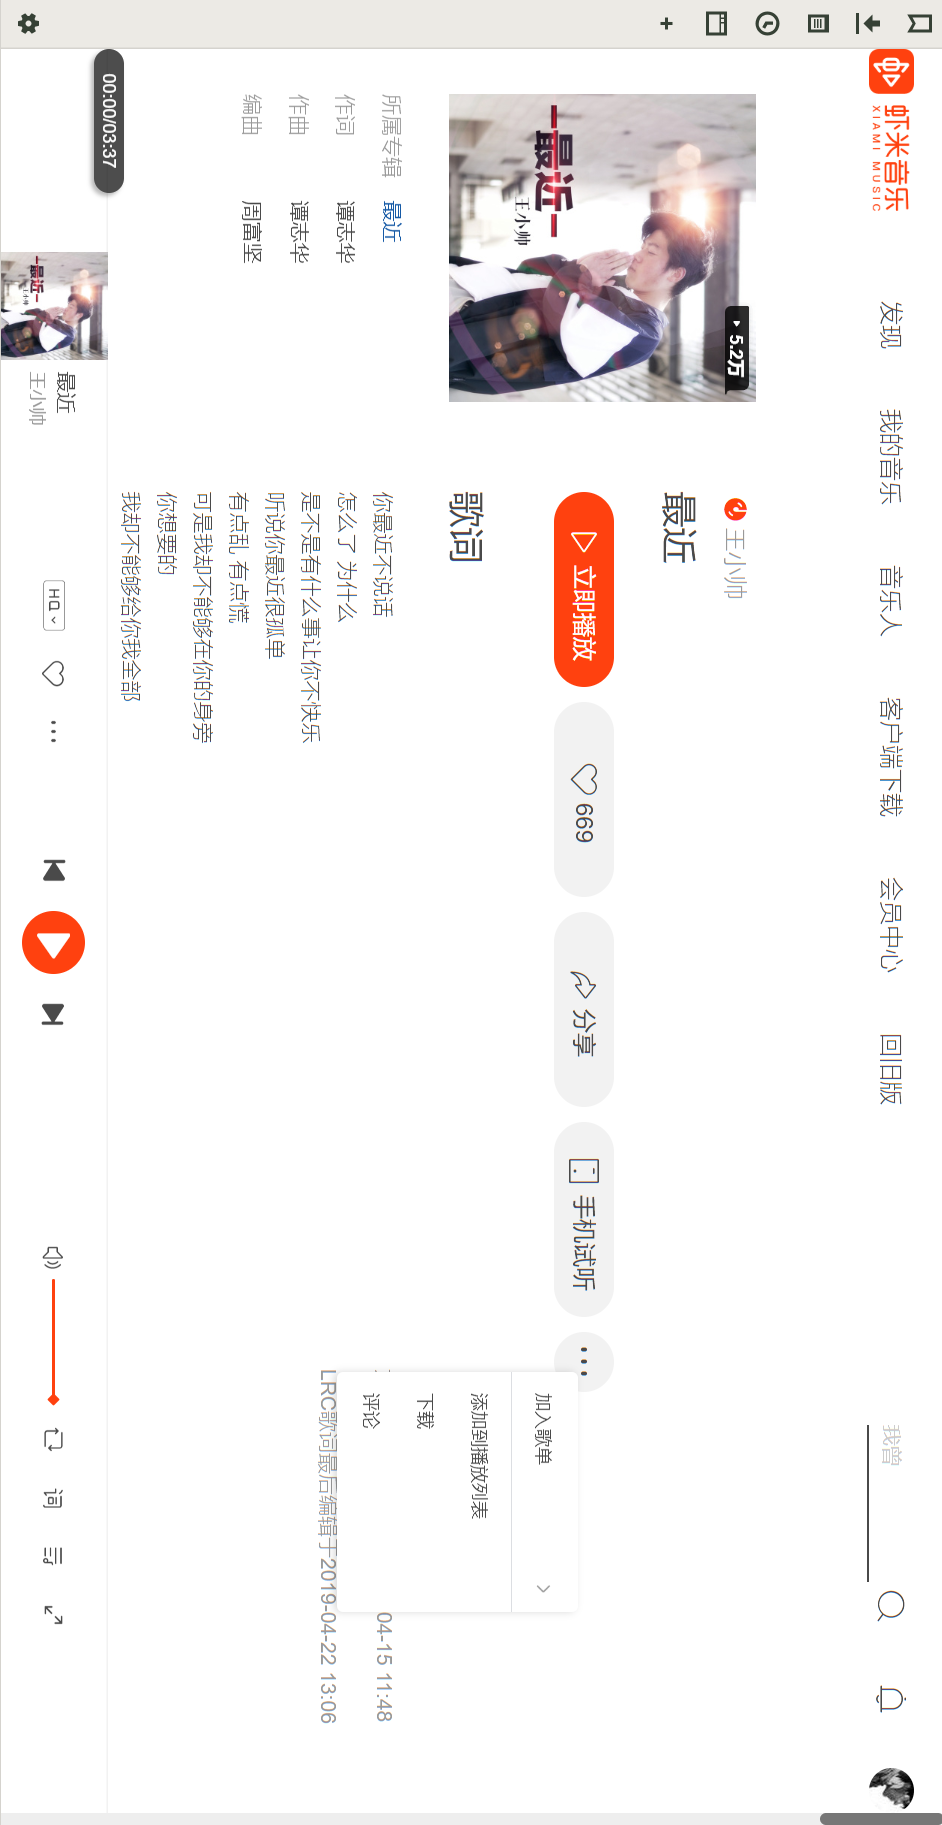
\includegraphics[width=0.5\textwidth]{./figures/capture14.png} 
			\end{sideways}
		\end{center}
		 \subsubsection{输入}
		 
		 用户在专辑页面、艺术家页面或风格页面点击某首歌曲的播放键,或者点击播放栏的歌曲切换按键
	  
	  
		 \subsubsection{处理}
		 
		 
		 
		 A. 输入数据的有效性检测:不需要进行有效性检测,因为输入是通过鼠标在对应区域点击引起中断造成的。
		 
		 B. 操作的确切次序:
		 \begin{adjustwidth}{2cm}{1cm}\qquad
			 \begin{itemize}
				 \item 中断事件发生
				 \item 调用监听函数
				 \item 将数据库查询请求传送到服务器端
				 \item 服务器通过查询获取音乐文件的url
				 \item 服务器通过tcp协议将文件传到客户端
				 \item 客户端接收到音乐文件,并利用动态网页图形界面控制音乐文件播放、暂停和切换
			 \end{itemize}		
		 \end{adjustwidth}
		  
		 
		 C. 对异常情况的回应,例如:
		 \begin{adjustwidth}{2cm}{1cm}\qquad
			 \begin{itemize}
				 \item 溢出
				 \item 通信失败
				 \item 错误处理
			 \end{itemize}		
		 \end{adjustwidth}
		 
			 发生以上错误时,函数体向网页返回错误代码,网页打印相应错误信息
		 
D. 通过过程性sql指令向数据库传送查询请求
				 
		 E. 对输出数据的有效性检测:
		 
		 在监听函数接收到数据库传送过来的数据后,首先进行合法性检测,如果合法则令网页正常显示;如果数据不合法或不安全——返回错误代码,让网页打印错误信息;
		 
		 \subsubsection{输出}
		 \begin{itemize}
			 \item	输出:用户档案数据库一个表项
			 \item	数量:1
			 \item	度量单位:条
			 \item	时序:无
			 \item	包含精确度和容忍度的有效输出范围:无
			 \item	对非法值的处理:打印错误信息
			 \item	错误消息:当输出不合法时,打印网页不存在或者输入信息错误;
			\end{itemize}
			详细描述:如果该音乐文件在服务器端确实存在,那么服务器将音乐文件传输到客户端,并通过动态网页播放音乐;




			\subsection{URS\_Download\_F016 在线音乐下载}
			\subsubsection{介绍}
		 
			前提条件:用户必须登录,并且处在专辑页面、艺术家页面或风格页面等可以直接点击单曲下载的功能页面中时。
			\begin{center}
				\begin{sideways} 
			   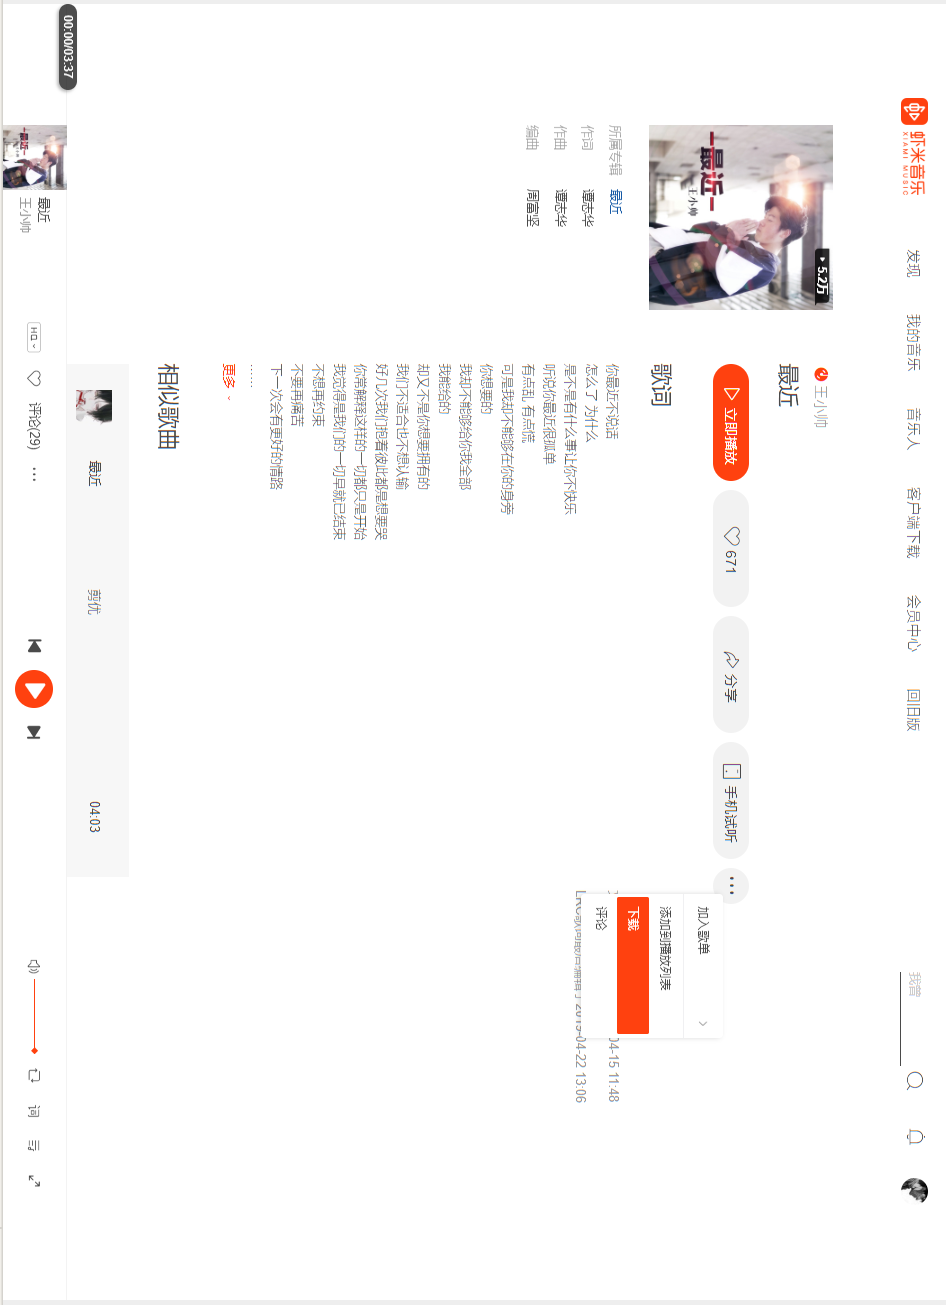
\includegraphics[width=0.5\textwidth]{./figures/capture18.png} 
				\end{sideways}
			\end{center}
			\subsubsection{输入}
			
			用户在专辑页面、艺术家页面或风格页面点击某首歌曲的下载键,或者点击播放页面的下载键
		 
		 
			\subsubsection{处理}
			
			
			
			A. 输入数据的有效性检测:不需要进行有效性检测,因为输入是通过鼠标在对应区域点击引起中断造成的。
			
			B. 操作的确切次序:
			\begin{adjustwidth}{2cm}{1cm}\qquad
				\begin{itemize}
					\item 中断事件发生
					\item 调用监听函数
					\item 将数据库查询请求传送到服务器端
					\item 服务器根据查询请求获取音乐文件的url,并检查用户是否购买该音乐
					\item 服务器通过tcp协议将文件传到客户端
					\item 客户端接收到音乐文件,并利用网页的下载插件将音乐固定到客户端的文件系统中
				\end{itemize}		
			\end{adjustwidth}
			 
			
			C. 对异常情况的回应,例如:
			\begin{adjustwidth}{2cm}{1cm}\qquad
				\begin{itemize}
					\item 溢出
					\item 通信失败
					\item 错误处理
				\end{itemize}		
			\end{adjustwidth}
			
				发生以上错误时,函数体向网页返回错误代码,网页打印相应错误信息
			
D. 通过过程性sql指令向数据库传送查询请求
					
			E. 对输出数据的有效性检测:
			
			在监听函数接收到数据库传送过来的数据后,首先进行合法性检测,如果合法则令网页正常显示;如果数据不合法或不安全——返回错误代码,让网页打印错误信息;
			
			\subsubsection{输出}
			\begin{itemize}
				\item	输出:用户档案数据库一个表项
				\item	数量:1
				\item	度量单位:条
				\item	时序:无
				\item	包含精确度和容忍度的有效输出范围:无
				\item	对非法值的处理:打印错误信息
				\item	错误消息:当输出不合法时,打印网页不存在或者输入信息错误;
			   \end{itemize}
			   详细描述:如果该音乐文件在服务器端确实存在,而且该用户有下载该歌曲的权限;那么服务器将音乐文件传输到客户端,并通过动态网页下载音乐;






			   \subsection{URS\_Creat-Sheet\_F017 创建新歌单}
			   \subsubsection{介绍}
			   
			   \begin{center}
				\begin{sideways} 
			   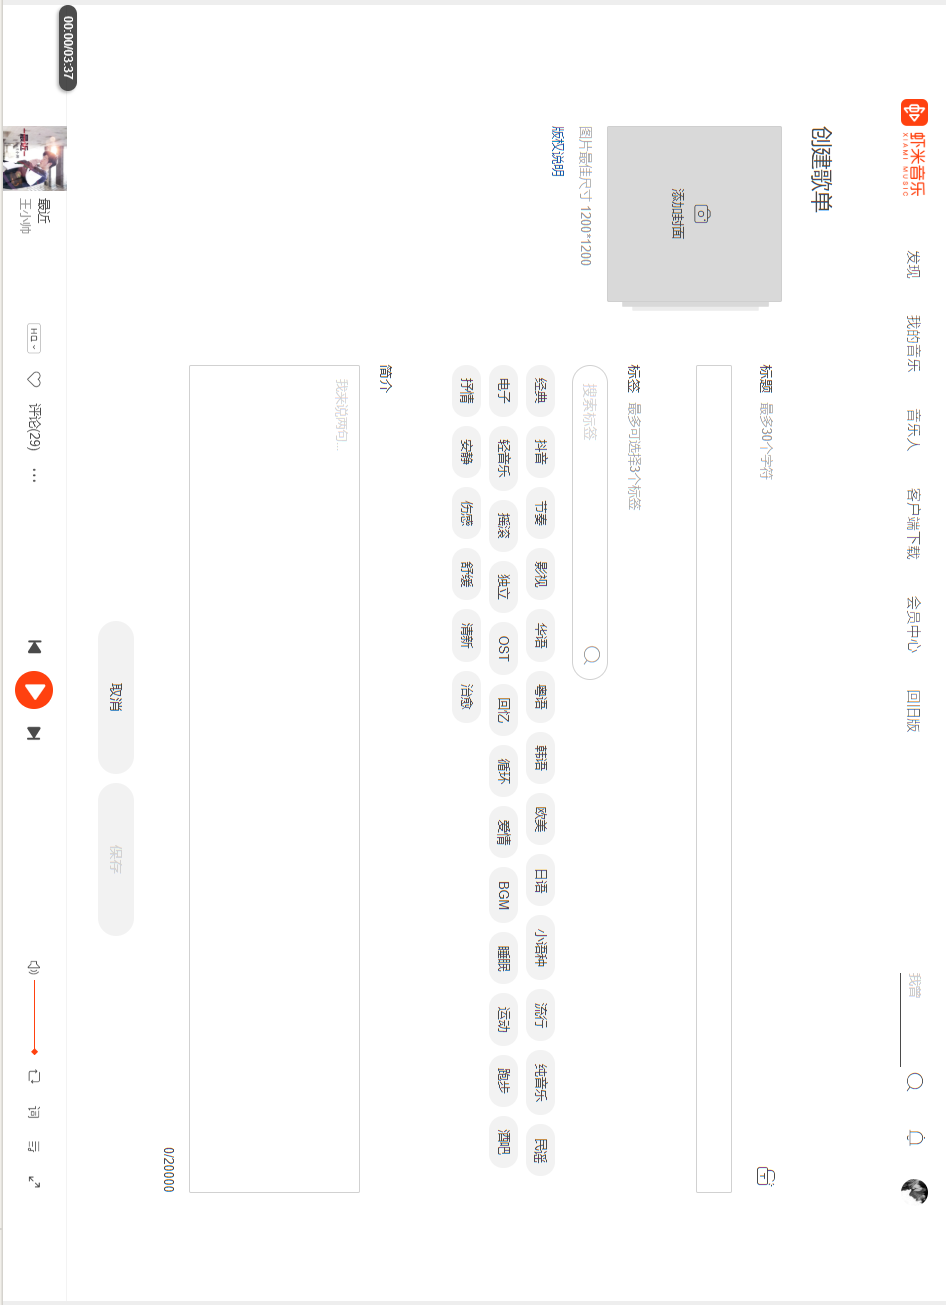
\includegraphics[width=0.5\textwidth]{./figures/capture16.png} 
				\end{sideways}
			\end{center}
			   \subsubsection{输入}
			   前提条件:用户必须登录,并且处在专辑页面、风格页面、歌单页面等可以直接将若干歌曲导入歌单的功能页面中,或者直接通过播放栏中的歌单创建按钮创建一个空歌单。
			
			   输入:用户在相应页面点击“导入歌单”或者“创建歌单”
			   
			   \subsubsection{处理}
			   
			
			   
			   A. 输入数据的有效性检测:不需要进行有效性检测,因为输入是通过鼠标在对应区域点击引起中断造成的。
			   
			   B. 操作的确切次序:
			   \begin{adjustwidth}{2cm}{1cm}\qquad
				   \begin{itemize}
					   \item 中断事件发生
					   \item 调用监听函数
					   \item 用户可以输入歌单名称,歌单介绍等相关信息
					   \item 输入完毕后,单击“完成”以完成操作
					   \item 将输入文本转化为数据库更新命令,传送到服务器端;同时将导入歌单的专辑、风格或者歌单的id也传输过去等数据
					   \item 服务器在音乐单表和歌单表、音乐关系表中添加相应表项
					   \item 服务器回送数据到客户端,刷新网页
				   \end{itemize}		
			   \end{adjustwidth}
				
			   
			   C. 对异常情况的回应,例如:
			   \begin{adjustwidth}{2cm}{1cm}\qquad
				   \begin{itemize}
					   \item 溢出
					   \item 通信失败
					   \item 错误处理
				   \end{itemize}		
			   \end{adjustwidth}
			   
				   发生以上错误时,函数体向网页返回错误代码,网页打印相应错误信息
			   D. 通过过程性sql指令向服务器传输命令,通过tcp协议传输数据
					   
			   E. 对输出数据的有效性检测:
			   
			   在监听函数接收到数据库传送过来的数据后,首先进行合法性检测,如果合法则令网页正常显示;如果数据不合法或不安全——返回错误代码,让网页打印错误信息;
			   
			   \subsubsection{输出}
			   \begin{itemize}
				   \item	输出:动态网页显示
				   \item	数量:1
				   \item	度量单位:页
				   \item	时序:无
				   \item	包含精确度和容忍度的有效输出范围:无
				   \item	对非法值的处理:打印错误信息
				   \item	错误消息:当输出不合法时,打印网页不存在或者输入信息错误;
				  \end{itemize}
				详细描述:执行操作后,将更新并保存对歌单的更改,并通过浏览器打印成功消息,告知用户修改已完成。
			




				\subsection{URS\_Add-Songs\_F018 添加歌曲到歌单}
				  \subsubsection{介绍}
			   
				  \begin{center}
				   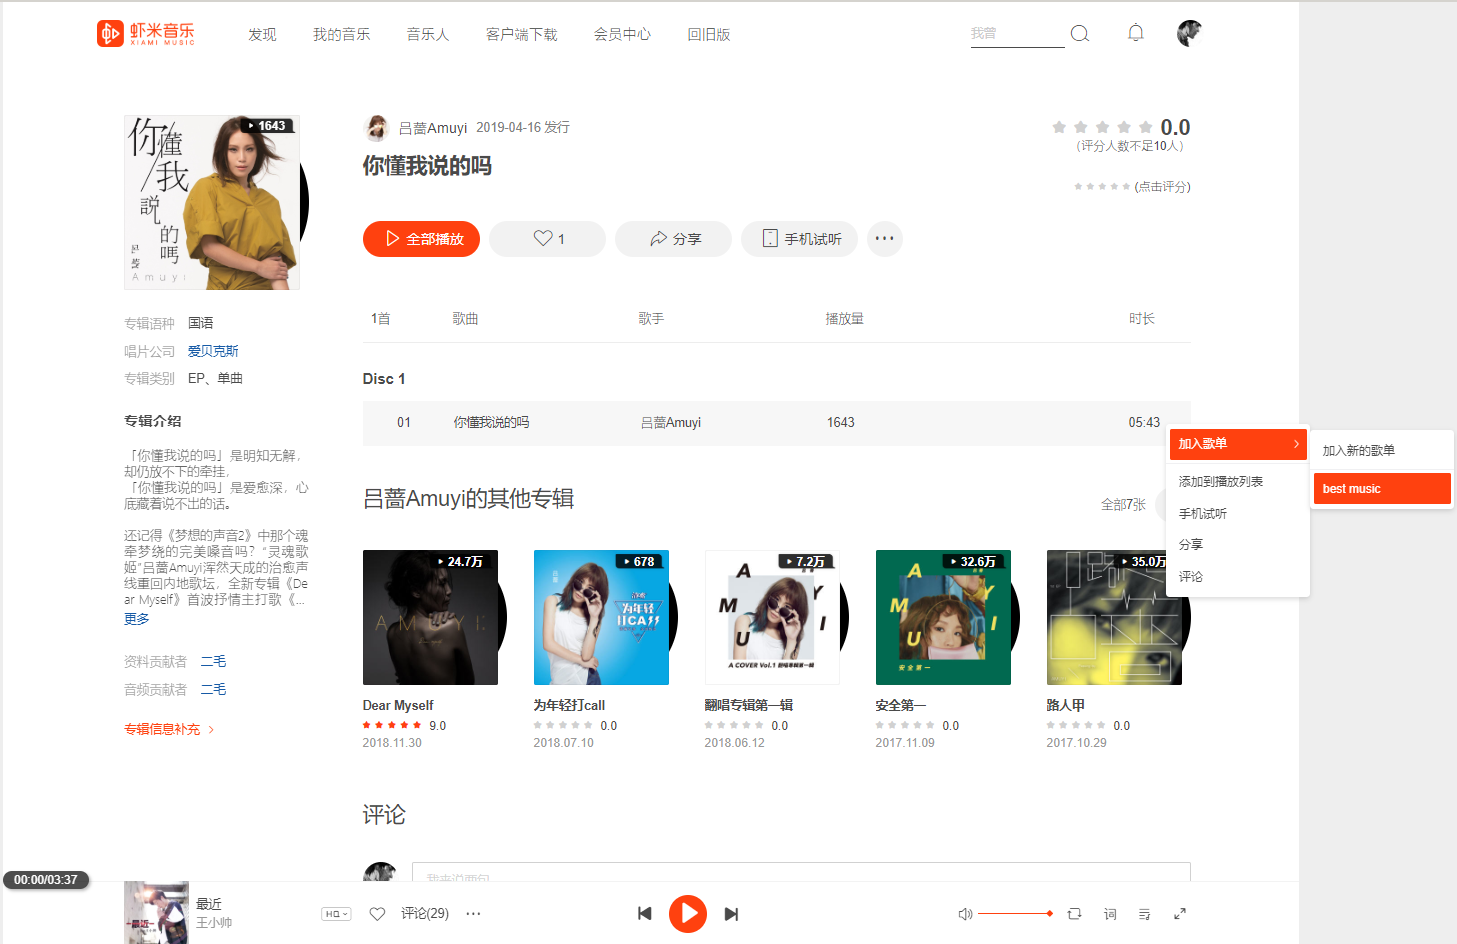
\includegraphics[width=0.5\textwidth]{./figures/capture17.png} 
	
				\end{center}
				  \subsubsection{输入}
				  前提条件:用户必须登录,并且处在专辑页面、艺术家页面或风格页面等可以直接点击单曲添加到歌单的页面;
			   
				  输入:用户点击某单曲,将单曲添加到指定歌单
				  
				  \subsubsection{处理}
				  
			   
				  
				  A. 输入数据的有效性检测:不需要进行有效性检测,因为输入是通过鼠标在对应区域点击引起中断造成的。
				  
				  B. 操作的确切次序:
				  \begin{adjustwidth}{2cm}{1cm}\qquad
					  \begin{itemize}
						  \item 中断事件发生
						  \item 调用监听函数
						  \item 用户选定欲添加的歌单
						  \item 输入完毕后,单击“完成”以完成操作
						  \item 将输入文本转化为数据库更新命令,传送到服务器端
						  \item 更新音乐关系表
						  \item 服务器回送数据到客户端,刷新网页
					  \end{itemize}		
				  \end{adjustwidth}
				   
				  
				  C. 对异常情况的回应,例如:
				  \begin{adjustwidth}{2cm}{1cm}\qquad
					  \begin{itemize}
						  \item 溢出
						  \item 通信失败
						  \item 错误处理
					  \end{itemize}		
				  \end{adjustwidth}
				  
					  发生以上错误时,函数体向网页返回错误代码,网页打印相应错误信息
				  D. 通过过程性sql指令向服务器传输命令
						  
				  E. 对输出数据的有效性检测:
				  
				  在监听函数接收到数据库传送过来的数据后,首先进行合法性检测,如果合法则令网页正常显示;如果数据不合法或不安全——返回错误代码,让网页打印错误信息;
				  
				  \subsubsection{输出}
				  \begin{itemize}
					  \item	输出:动态网页显示
					  \item	数量:1
					  \item	度量单位:页
					  \item	时序:无
					  \item	包含精确度和容忍度的有效输出范围:无
					  \item	对非法值的处理:打印错误信息
					  \item	错误消息:当输出不合法时,打印网页不存在或者输入信息错误;
					 \end{itemize}
					 详细描述:执行操作后,将更新并保存对音乐关系表的更改,并通过浏览器打印成功消息,告知用户修改已完成。




			
					 \subsection{URS\_Delete-Sheet\_F019 删除歌单}
				  \subsubsection{介绍}
				  
				  \begin{center}
					\begin{sideways} 
				   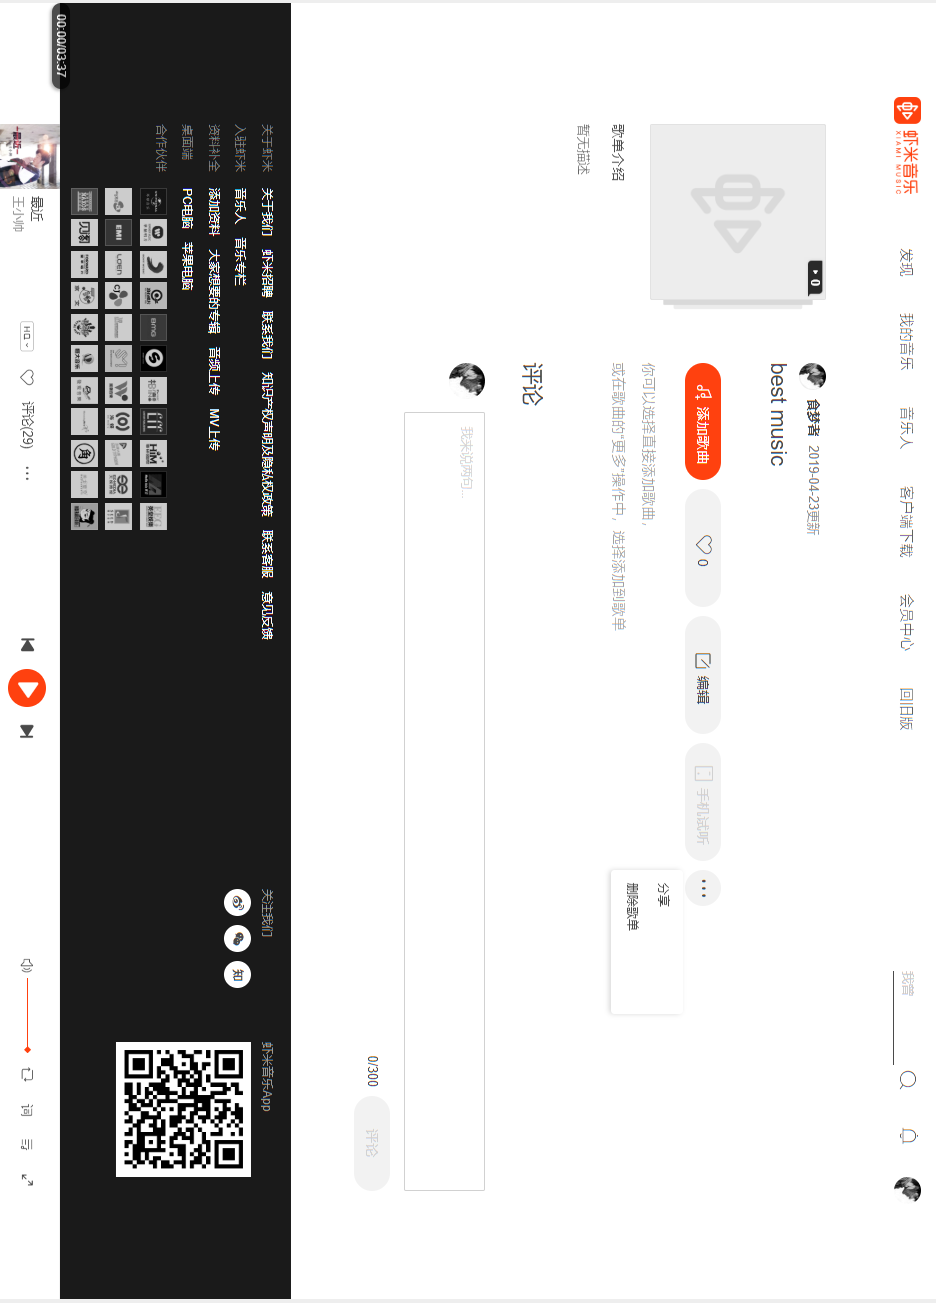
\includegraphics[width=0.5\textwidth]{./figures/capture20.png} 
					\end{sideways}

				\end{center}
				  前提条件:用户必须登录,并进入歌单页面才能删除歌单
			   
				  输入:用户进入歌单页面,然后单击“删除”按钮。
				  
				  \subsubsection{处理}
				  
			   
				  
				  A. 输入数据的有效性检测:不需要进行有效性检测,因为输入是通过鼠标在对应区域点击引起中断造成的。
				  
				  B. 操作的确切次序:
				  \begin{adjustwidth}{2cm}{1cm}\qquad
					  \begin{itemize}
						  \item 中断事件发生
						  \item 调用监听函数
						  \item 管理员可以输入名称和必要的详细信息
						  \item 输入完毕后,单击“删除”以完成操作
						  \item 将输入文本转化为数据库删除命令,传送到服务器端
						  \item 服务器在音乐单表中删除条目,级联删除所有引用该条目的条目
						  \item 服务器回送数据到客户端,刷新网页
					  \end{itemize}		
				  \end{adjustwidth}
				   
				  
				  C. 对异常情况的回应,例如:
				  \begin{adjustwidth}{2cm}{1cm}\qquad
					  \begin{itemize}
						  \item 溢出
						  \item 通信失败
						  \item 错误处理
					  \end{itemize}		
				  \end{adjustwidth}
				  
					  发生以上错误时,函数体向网页返回错误代码,网页打印相应错误信息
				  D. 通过过程性sql指令向服务器传输命令
						  
				  E. 对输出数据的有效性检测:
				  
				  在监听函数接收到数据库传送过来的数据后,首先进行合法性检测,如果合法则令网页正常显示;如果数据不合法或不安全——返回错误代码,让网页打印错误信息;
				  
				  \subsubsection{输出}
				  \begin{itemize}
					  \item	输出:动态网页显示
					  \item	数量:1
					  \item	度量单位:页
					  \item	时序:无
					  \item	包含精确度和容忍度的有效输出范围:无
					  \item	对非法值的处理:打印错误信息
					  \item	错误消息:当输出不合法时,打印网页不存在或者输入信息错误;
					 \end{itemize}
					 详细描述:执行操作后,将更新并保存对目录的更改,并通过浏览器打印成功消息,告知用户修改已完成。



			
对于管理员,应该能够满足以下功能

\subsection{URS\_Land\_F020 系统登录需求}

\subsubsection{介绍}
现此目的以启用系统管理员身份验证,必须为现有客户保留有效的帐户。

\subsubsection{输入}

输入:用户将通过键盘输入用户名和密码。

\subsubsection{处理}



A. 输入数据的有效性检测:不需要进行有效性检测,因为输入是通过鼠标在对应区域点击引起中断造成的。

B. 操作的确切次序:
\begin{adjustwidth}{2cm}{1cm}\qquad
	\begin{itemize}
		\item 中断事件发生
		\item 调用监听函数
		\item 用户可以输入账户和密码
		\item 文本输入完毕后,单击“Login”按钮
		\item 将输入文本转化为数据库查询,传送到服务器端
		\item 服务器验证用户名和密码是否匹配
		\item 若匹配,检查用户档案数据库中的角色条目
		\item 如果服务器确认用户拥有管理员权限,那么用户被归类为管理员
		\item 服务器回送数据到客户端,使客户端网页重定向到系统管理员页面
	\end{itemize}		
\end{adjustwidth}
 

C. 对异常情况的回应,例如:
\begin{adjustwidth}{2cm}{1cm}\qquad
	\begin{itemize}
		\item 溢出
		\item 通信失败
		\item 错误处理
	\end{itemize}		
\end{adjustwidth}

	发生以上错误时,函数体向网页返回错误代码,网页打印相应错误信息
D. 通过tcp协议向服务器传输有关数据
		
E. 对输出数据的有效性检测:

在监听函数接收到数据库传送过来的数据后,首先进行合法性检测,如果合法则令网页正常显示;如果数据不合法或不安全——返回错误代码,让网页打印错误信息;

\subsubsection{输出}
\begin{itemize}
	\item	输出:动态网页显示
	\item	数量:1
	\item	度量单位:页
	\item	时序:无
	\item	包含精确度和容忍度的有效输出范围:无
	\item	对非法值的处理:打印错误信息
	\item	错误消息:当输出不合法时,打印网页不存在或者输入信息错误;
   \end{itemize}
   详细描述:如果用户名或密码无效,将显示相应的错误消息,并要求用户重新输入用户名和密码。
   如果用户输入有效,将显示默认页面。
   如果用户被归类为管理员,则他/她将被重定向到管理员页面,其中他/她可以更新类别详细信息并查看客户订单。





   \subsection{URS\_Creat-index\_F021 为目录创建和添加新类别(专辑 / 艺术家 / 流派 、单曲)}
   实现此功能是为了系统管理员能够执行下列任务
   \subsubsection{介绍}


   \subsubsection{输入}
   前提条件:管理员必须登录才能创建和添加新类型。并且管理员必须先跳转到添加页面

   输入:管理员将输入名称和必要的详细信息,以便为目录创建新的流派或类别,然后单击“添加”按钮以完成操作。
   
   \subsubsection{处理}
   

   
   A. 输入数据的有效性检测:不需要进行有效性检测,因为输入是通过鼠标在对应区域点击引起中断造成的。
   
   B. 操作的确切次序:
   \begin{adjustwidth}{2cm}{1cm}\qquad
	   \begin{itemize}
		   \item 中断事件发生
		   \item 调用监听函数
		   \item 管理员可以输入名称和必要的详细信息
		   \item 输入完毕后,单击“按钮”以完成操作
		   \item 将输入文本转化为数据库更新命令,传送到服务器端
		   \item 服务器验证用户是否具有管理员权限,然后在目录数据库中添加新的类别
		   \item 服务器回送数据到客户端,刷新网页
	   \end{itemize}		
   \end{adjustwidth}
	
   
   C. 对异常情况的回应,例如:
   \begin{adjustwidth}{2cm}{1cm}\qquad
	   \begin{itemize}
		   \item 溢出
		   \item 通信失败
		   \item 错误处理
	   \end{itemize}		
   \end{adjustwidth}
   
	   发生以上错误时,函数体向网页返回错误代码,网页打印相应错误信息
   D. 通过过程性sql指令向服务器传输命令
		   
   E. 对输出数据的有效性检测:
   
   在监听函数接收到数据库传送过来的数据后,首先进行合法性检测,如果合法则令网页正常显示;如果数据不合法或不安全——返回错误代码,让网页打印错误信息;
   
   \subsubsection{输出}
   \begin{itemize}
	   \item	输出:动态网页显示
	   \item	数量:1
	   \item	度量单位:页
	   \item	时序:无
	   \item	包含精确度和容忍度的有效输出范围:无
	   \item	对非法值的处理:打印错误信息
	   \item	错误消息:当输出不合法时,打印网页不存在或者输入信息错误;
	  \end{itemize}
	  详细描述:执行操作后,将更新并保存对目录的更改,并通过浏览器打印成功消息,告知用户修改已完成。



	  \subsection{URS\_Delete-index\_F022 为目录删除类别(专辑 / 艺术家 / 流派 / 单曲 )}
	  \subsubsection{介绍}
	  
	  \subsubsection{输入}
	  前提条件:管理员必须登录才能删除新类型,目录中必须至少有一种类型。管理员首先从管理页面跳转到删除页面;
   
	  输入:管理员将指定要从目录中删除的类型/类别,然后单击“删除”按钮。
	  
	  \subsubsection{处理}
	  
   
	  
	  A. 输入数据的有效性检测:不需要进行有效性检测,因为输入是通过鼠标在对应区域点击引起中断造成的。
	  
	  B. 操作的确切次序:
	  \begin{adjustwidth}{2cm}{1cm}\qquad
		  \begin{itemize}
			  \item 中断事件发生
			  \item 调用监听函数
			  \item 管理员可以输入名称和必要的详细信息
			  \item 输入完毕后,单击“删除”以完成操作
			  \item 将输入文本转化为数据库删除命令,传送到服务器端
			  \item 服务器验证用户是否具有管理员权限,然后在目录数据库中删除条目
			  \item 服务器回送数据到客户端,刷新网页
		  \end{itemize}		
	  \end{adjustwidth}
	   
	  
	  C. 对异常情况的回应,例如:
	  \begin{adjustwidth}{2cm}{1cm}\qquad
		  \begin{itemize}
			  \item 溢出
			  \item 通信失败
			  \item 错误处理
		  \end{itemize}		
	  \end{adjustwidth}
	  
		  发生以上错误时,函数体向网页返回错误代码,网页打印相应错误信息
	  D. 通过过程性sql指令向服务器传输命令
			  
	  E. 对输出数据的有效性检测:
	  
	  在监听函数接收到数据库传送过来的数据后,首先进行合法性检测,如果合法则令网页正常显示;如果数据不合法或不安全——返回错误代码,让网页打印错误信息;
	  
	  \subsubsection{输出}
	  \begin{itemize}
		  \item	输出:动态网页显示
		  \item	数量:1
		  \item	度量单位:页
		  \item	时序:无
		  \item	包含精确度和容忍度的有效输出范围:无
		  \item	对非法值的处理:打印错误信息
		  \item	错误消息:当输出不合法时,打印网页不存在或者输入信息错误;
		 \end{itemize}
		 详细描述:执行操作后,将更新并保存对目录的更改,并通过浏览器打印成功消息,告知用户修改已完成。








			   
\section{性能需求}
该应用程序将用于客户端缓存以获取用户输入,以减少Web服务器的负载。此外,JavaScript将用于实现客户端验证,以减轻服务器端的负载。
系统负载主要为查询数据库中的数据造成的开销。音乐文件大小应为10MB左右。服务器和客户端之间的最大响应时间和数据传输时间约为2分钟,每个事务的典型值为56kbps。
总共有大约100个用户。为了实现最高性能并适应所有用户连接,系统将使用Microsoft SQL服务器而不是测试服务器MSDE构建,该服务器仅接受八个并发用户连接请求。建议所有用户使用宽带连接访问系统,以提高性能。


静态的量化需求可能包括:

A. 支持的终端数目,最多100个用户;

B. 支持的同时使用的用户数目,仅能同时接受八个用户的并发访问;

C.处理的文件和记录的数目。音乐文件的大小应该每个在10MB左右,音乐文件的总数应该不超过五千首;

D.表和文件的大小:音乐关系表平均来说可能有十万个左右的表项,其余的数据库表单的表项数量应该都在数千左右;储存音乐文件总容量大概为50GB;

动态的量化需求可能包括:

A. 在正常和峰值工作量条件下特定时间段(如一小时),峰值为8个用户同时提出批量传输音乐的请求时,但是以本组预设服务器的能力能够完成,不成问题;




\section{外部接口需求}

\subsection{用户接口}
<The interface of the system with the User and vice versa should be explained in detail. >

详细描述系统与用户之间的接口


这应描述下述内容:

% A. 对每种人机界面,软件所必须支持的特性。例如,如果系统用户通过一个显示终端进行操作,那么应包含下述内容:
% 要求的屏幕格式
% 页面规划及报告或菜单的内容
% 输入和输出的相关时序
% 一些组合功能键的用法
A:
要求的屏幕格式:1080*1920(像素点)

页面规划内容:
最上方为导航栏(可以跳转到购物车,搜索页面,分享消息页,信息编辑页面)
左侧为类别划分(可以跳转到推荐页面,排行榜,分类页面)
最下方为播放栏(单击播放栏可以进入播放页面)
输入和输出的相关时序:接受鼠标输入,获取屏幕输出
一些组合功能键的用法:无

B. 与系统用户接口使用相关的所有方面。这可能只是一个简单的关于系统怎样展示给用户而该做什么和不该做什么的列表。例如提供关于长或短错误消息选项。和所有其它需求一样,这些需求也应能被检验,例如,四级打字员经一小时的培训后能在Z分钟内完成功能X,而不是一个打字员能完成功能X。

普通用户只用于以下权限:打开自己的购物车,打开歌单,按关键字搜索实体,获得排行榜歌单,获得系统推荐歌单,查看其它用户给自己推送的分享,向其它用户推送分享,从目录查看音乐/专辑/艺人;
管理员除了以上权限还拥有:删除单曲/专辑/艺人/风格的权限,上传单曲,添加专辑/艺人/风格的权限,向其它用户赋予管理员权限的权限;
\subsection{软件接口}


在此应描述如何使用其它(必需的)软件产品(例如,数据管理系统,操作系统,或算法工具包),以及与其它应用系统的接口(例如,协议处理系统和数据库管理系统之间的接口)。

% 对每个必需的软件产品,应提供下列信息:
% A.	名字
% B.	助记符
% C.	版本号
% D.	来源

% 对每个接口,本部分应:
% 所有用户界面都是ASP.NET生成的Web页面。
% 为了访问系统,用户需要使用配备Internet Explorer的具有Internet可访问性的工作站。
% Microsoft .NET Framework也必须安装在同一台计算机上。

A.	名字:Active Server Pages
B.	助记符:ASP.net
C.  版本号:.NET Framework 4.8
D.	来源:通过官网下载

E. 功能:该软件生成客户端浏览器中的动态网页

F. 接口:请参见微软官方文档;

A.	名字:Internet Explorer
B.	助记符:IE
C.  版本号:11
D.	来源:通过官网下载

E. 功能:该软件用于渲染有ASP.NET生成的网页,并输出到屏幕

F. 接口:请参见微软官方文档;

A.	名字:Microsoft XML Web services flatform
B.	助记符:.NET
C.  版本号:4.0
D.	来源:通过官网下载

E. 功能:Microsoft .NET 平台提供创建 XML Web services 并将这些服务集成在一起之所需;换言之,为上述软件的正常运行提供必要的支持;

F. 接口:请参见微软官方文档;

\subsection{硬件接口}
请参考C\#官方文档;



\subsection{通讯接口}
本次开发中,笔者使用tcp协议作为数据传输的默认协议;
tcp协议的说明请参考tcp协议的官方文档(RFC793);
